\chapter{Results: \deploy Demonstration}
In this chapter, we demonstrate \deploy's capabilities
in \Cyclus transition scenario simulations.  
This chapter has two sections: 
\begin{enumerate}
    \item \deploy demonstration for simple three-facility transition scenarios
    \item \deploy demonstration for a complex closed cycle transition scenario
\end{enumerate}

\section{\deploy Demonstration of Simple Transition Scenarios}
\label{sec:demo}

This section demonstrates \deploy's capability 
to effectively set up a simple transition scenario simulation 
for constant, linearly increasing, and 
sinusoidal power demand simulations.
These simulations are defined as \textit{simple} since 
they only include
three facility types: \texttt{source}, \texttt{reactor}, and 
\texttt{sink}. 
The simulations begin with ten \texttt{reactor} facilities 
(\texttt{reactor1} to \texttt{reactor10}). 
These reactors have staggered cycle lengths and lifetimes to prevent 
simultaneous refueling and to set up gradual decommissioning. 
\deploy is configured to deploy \texttt{new reactor} facilities
to meet the loss of power supply created by the decommissioning 
of the initial \texttt{reactor} facilities. 
Table \ref{tab:demonstrations} shows the 
\deploy input parameters for these simulations.
Figure \ref{fig:powerplots} shows the user-defined power demand curves 
driving deployment in three simulations. 

\begin{table}[]
    \caption{\deploy's input parameters for the simple constant, 
    linearly increasing, and sinusoidal power demand 
    transition scenarios.}
    \label{tab:demonstrations}
    \resizebox{1\textwidth}{!}{%
    \doublespacing
    \begin{tabular}{l|c|c|c}
    \hline
    &\multicolumn{3}{c}{\textbf{Simulation Description}}                                                                                                                                                                                                                                                       \\ \hline
    \multicolumn{1}{c|}{\textbf{Input Parameter}}                           & \multicolumn{1}{l|}{\textbf{Constant Power}}                                                                 & \textbf{\begin{tabular}[c]{@{}l@{}}Linearly Increasing \\ Power\end{tabular}}                  & \textbf{Sinusoidal Power}                                                                  \\ \hline
    Demand driving commodity                                       & \multicolumn{3}{c}{Power}                                                                                                                                                                                                                                                                                 \\ \hline 
    Demand equation [MW]                                               & \multicolumn{1}{l|}{10000}                                                                                & \begin{tabular}[c]{@{}l@{}}t\textless 40: 10000\\ t\textgreater{}=40: 250t\end{tabular} & 10000+ 1000$\sin(\pi*t/3)$                                                                 \\ \hline 
    Available Facilities                                           & \multicolumn{3}{c}{Source, Reactor, Sink}                                                                                                                                                                                                                                                                 \\ \hline
    Prediction method                                              & \multicolumn{1}{l|}{\begin{tabular}[c]{@{}l@{}}Power: \texttt{FFT}\\ Fuel: \texttt{MA}\\ Spent fuel: \texttt{MA}\end{tabular}}          & \begin{tabular}[c]{@{}l@{}}Power: FFT\\ Fuel: MA\\ Spent fuel: FFT\end{tabular}                & \begin{tabular}[c]{@{}l@{}}Power: HW\\ Fuel: MA\\ Spent fuel: FFT\end{tabular}             \\\hline 
    Deployment Driving Method                                      & \multicolumn{3}{c}{Installed Capacity}                                                                                                                                                                                                                                                                    \\ \hline
    Buffer type                                                    & \multicolumn{3}{c}{Absolute}                                                                                                                                                                                                                                                                              \\ \hline 
    Buffer size                                                    & \multicolumn{1}{l|}{\begin{tabular}[c]{@{}l@{}}Power: 3000 MW\\ Fuel: 0 kg \\ Spent fuel: 0 kg\end{tabular}} & \begin{tabular}[c]{@{}l@{}}Power: 2000 MW\\ Fuel: 1000 kg \\ Spent fuel: 0 kg\end{tabular}     & \begin{tabular}[c]{@{}l@{}}Power: 2000 MW\\ Fuel: 1000 kg \\ Spent fuel: 0 kg\end{tabular} \\ \hline
    \end{tabular}
    }
    \end{table}

    \begin{figure}[]
        \begin{center}
            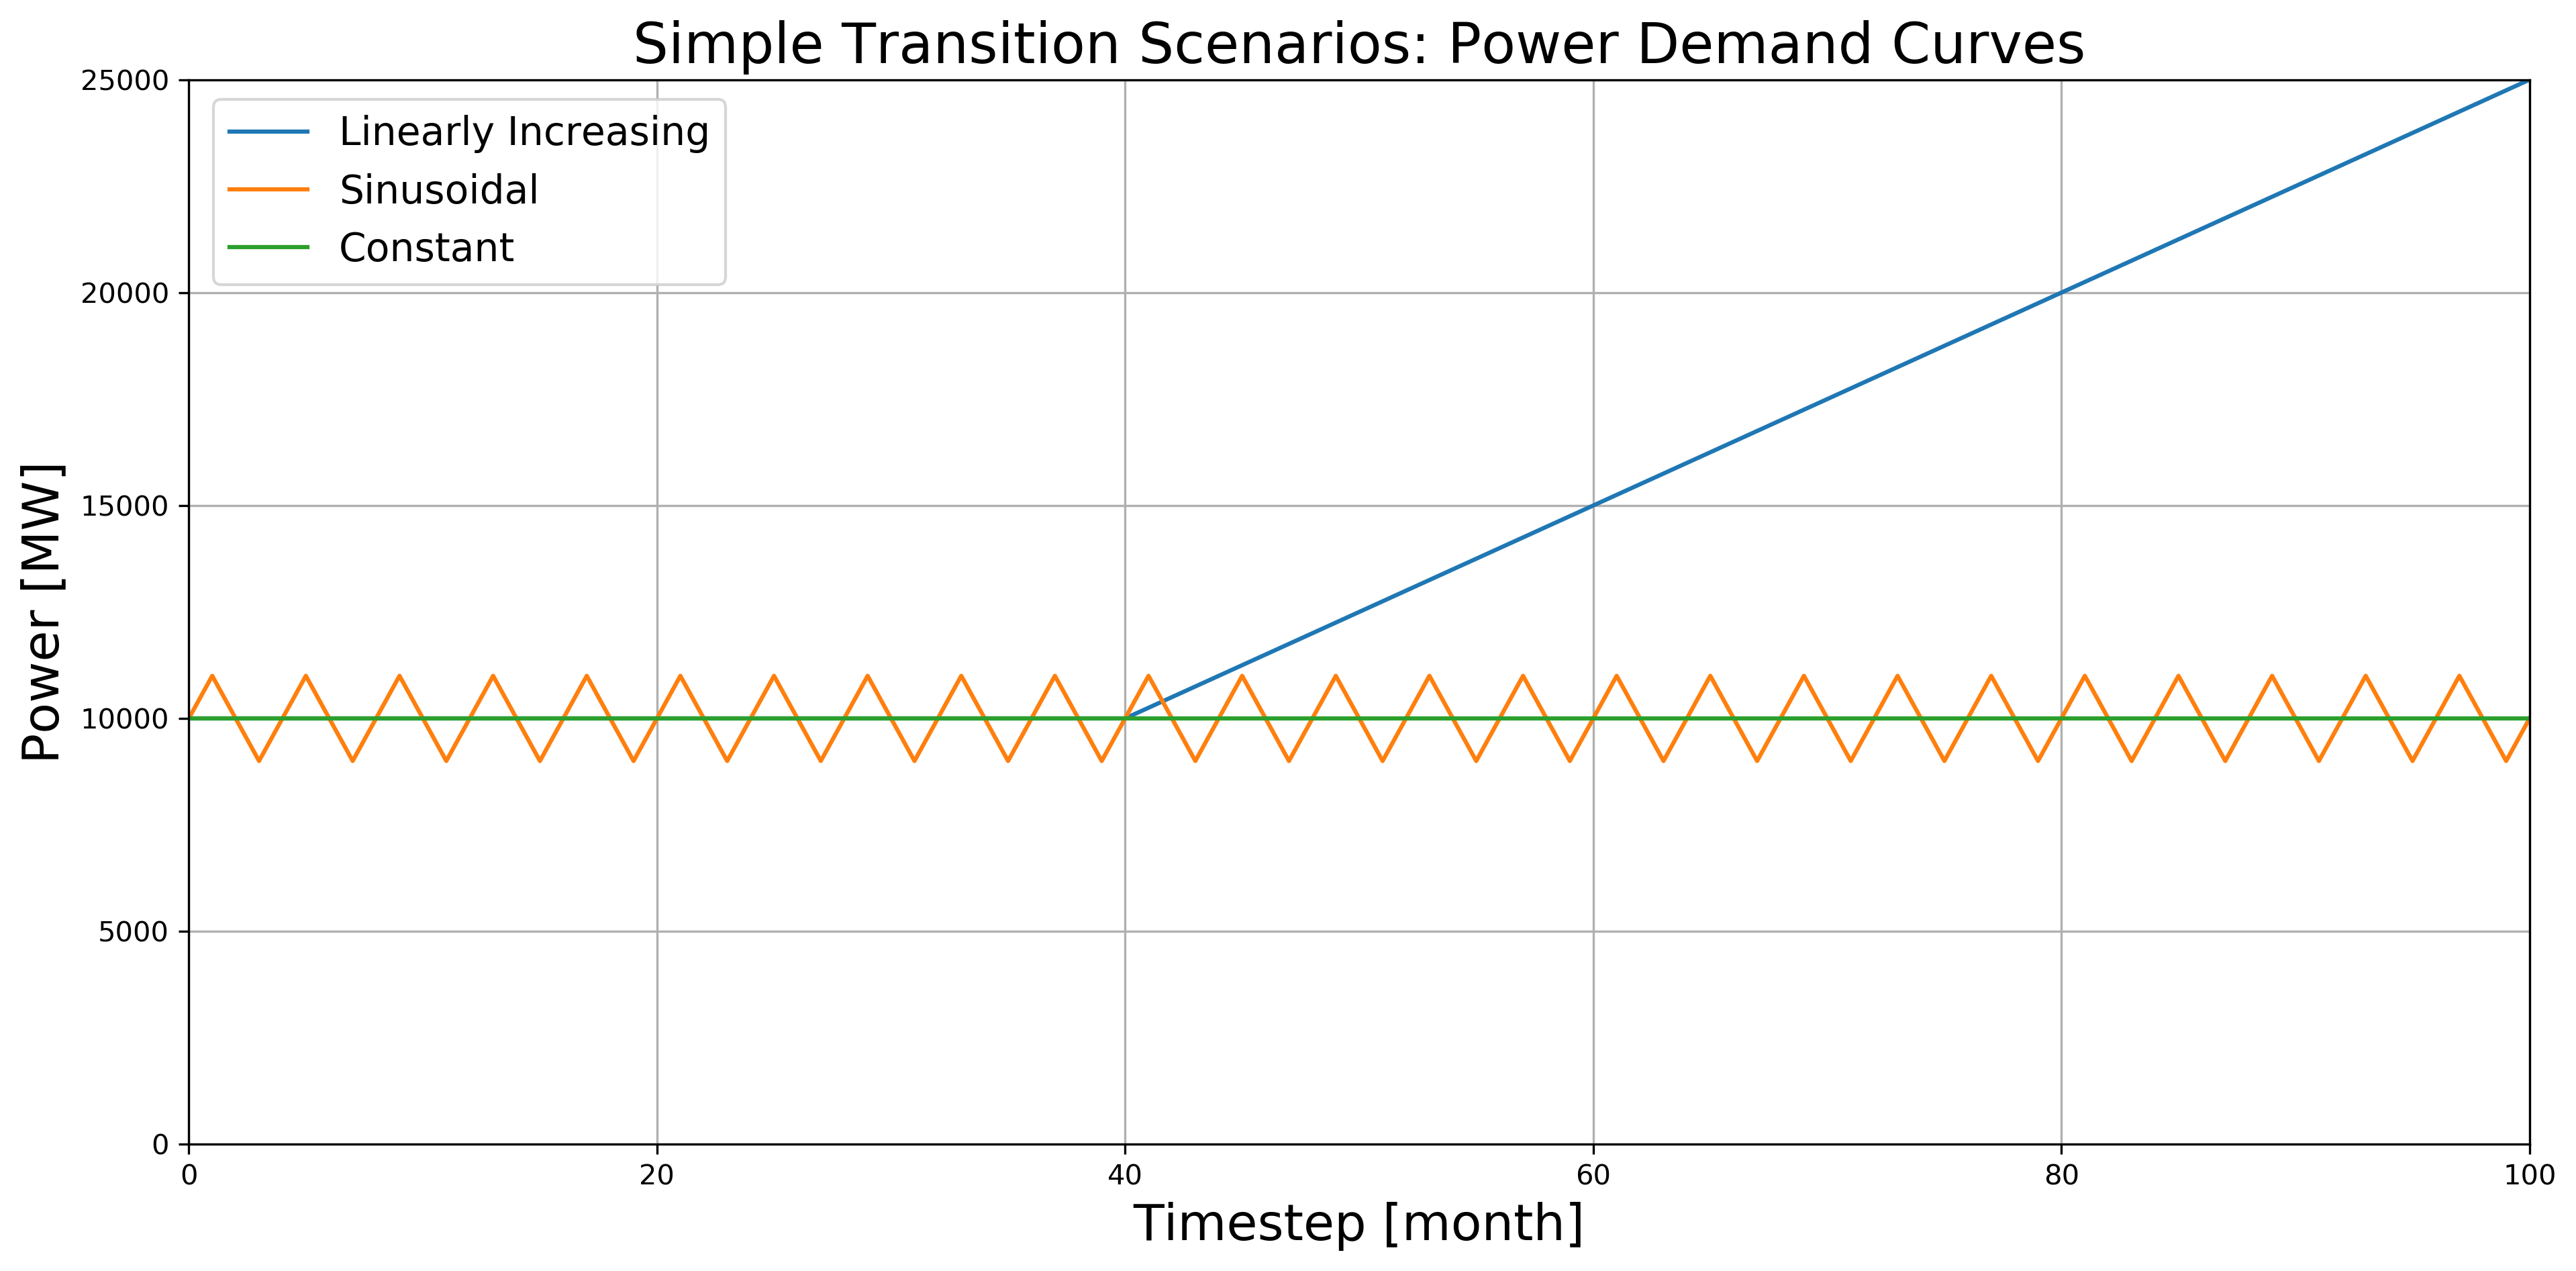
\includegraphics[scale=0.45]{./figures/powerplots.png}
        \end{center}
            \caption{Power demand curves for the simple constant, 
            linearly increasing, and sinusoidal power demand 
            transition scenarios.}
        \label{fig:powerplots}
    \end{figure}

\subsection{Simple Transition Scenario Simulation: Constant Demand}
Figures \ref{fig:constanttransition-power}, \ref{fig:constanttransition-fuel},
and \ref{fig:constanttransition-spentfuel} demonstrate \deploy's capability 
to deploy reactor and supporting facilities to minimize undersupply 
when meeting linearly increasing power demand and subsequent secondary 
commodities demand.  
Table \ref{tab:transition-scenario-results} shows the number of 
undersupplied timesteps. 
In Figure \ref{fig:constanttransition-power}, there exist no time steps 
in which the supply of power falls under demand, meeting the main 
objective of \deploy. 
By using the \texttt{FFT} method for 
predicting demand and setting the power supply buffer to 3000MW 
(the capacity of 3 reactors), the user minimizes the number of 
undersupplied timesteps for every commodity.

In Figure \ref{fig:constanttransition-fuel},
a large-throughput source facility is initially
deployed to meet the large initial fuel demand for the commissioning 
of ten reactors. 
Deployment of a large-throughput source facility for the 
first few time steps ensures \deploy does not deploy supporting
facilities that become redundant at later times in  
the simulation.
This reflects reality in which reactor manufacturers accumulate
an appropriate amount of fuel inventory before starting 
up reactors. 

    \begin{figure}[]
        \centering
        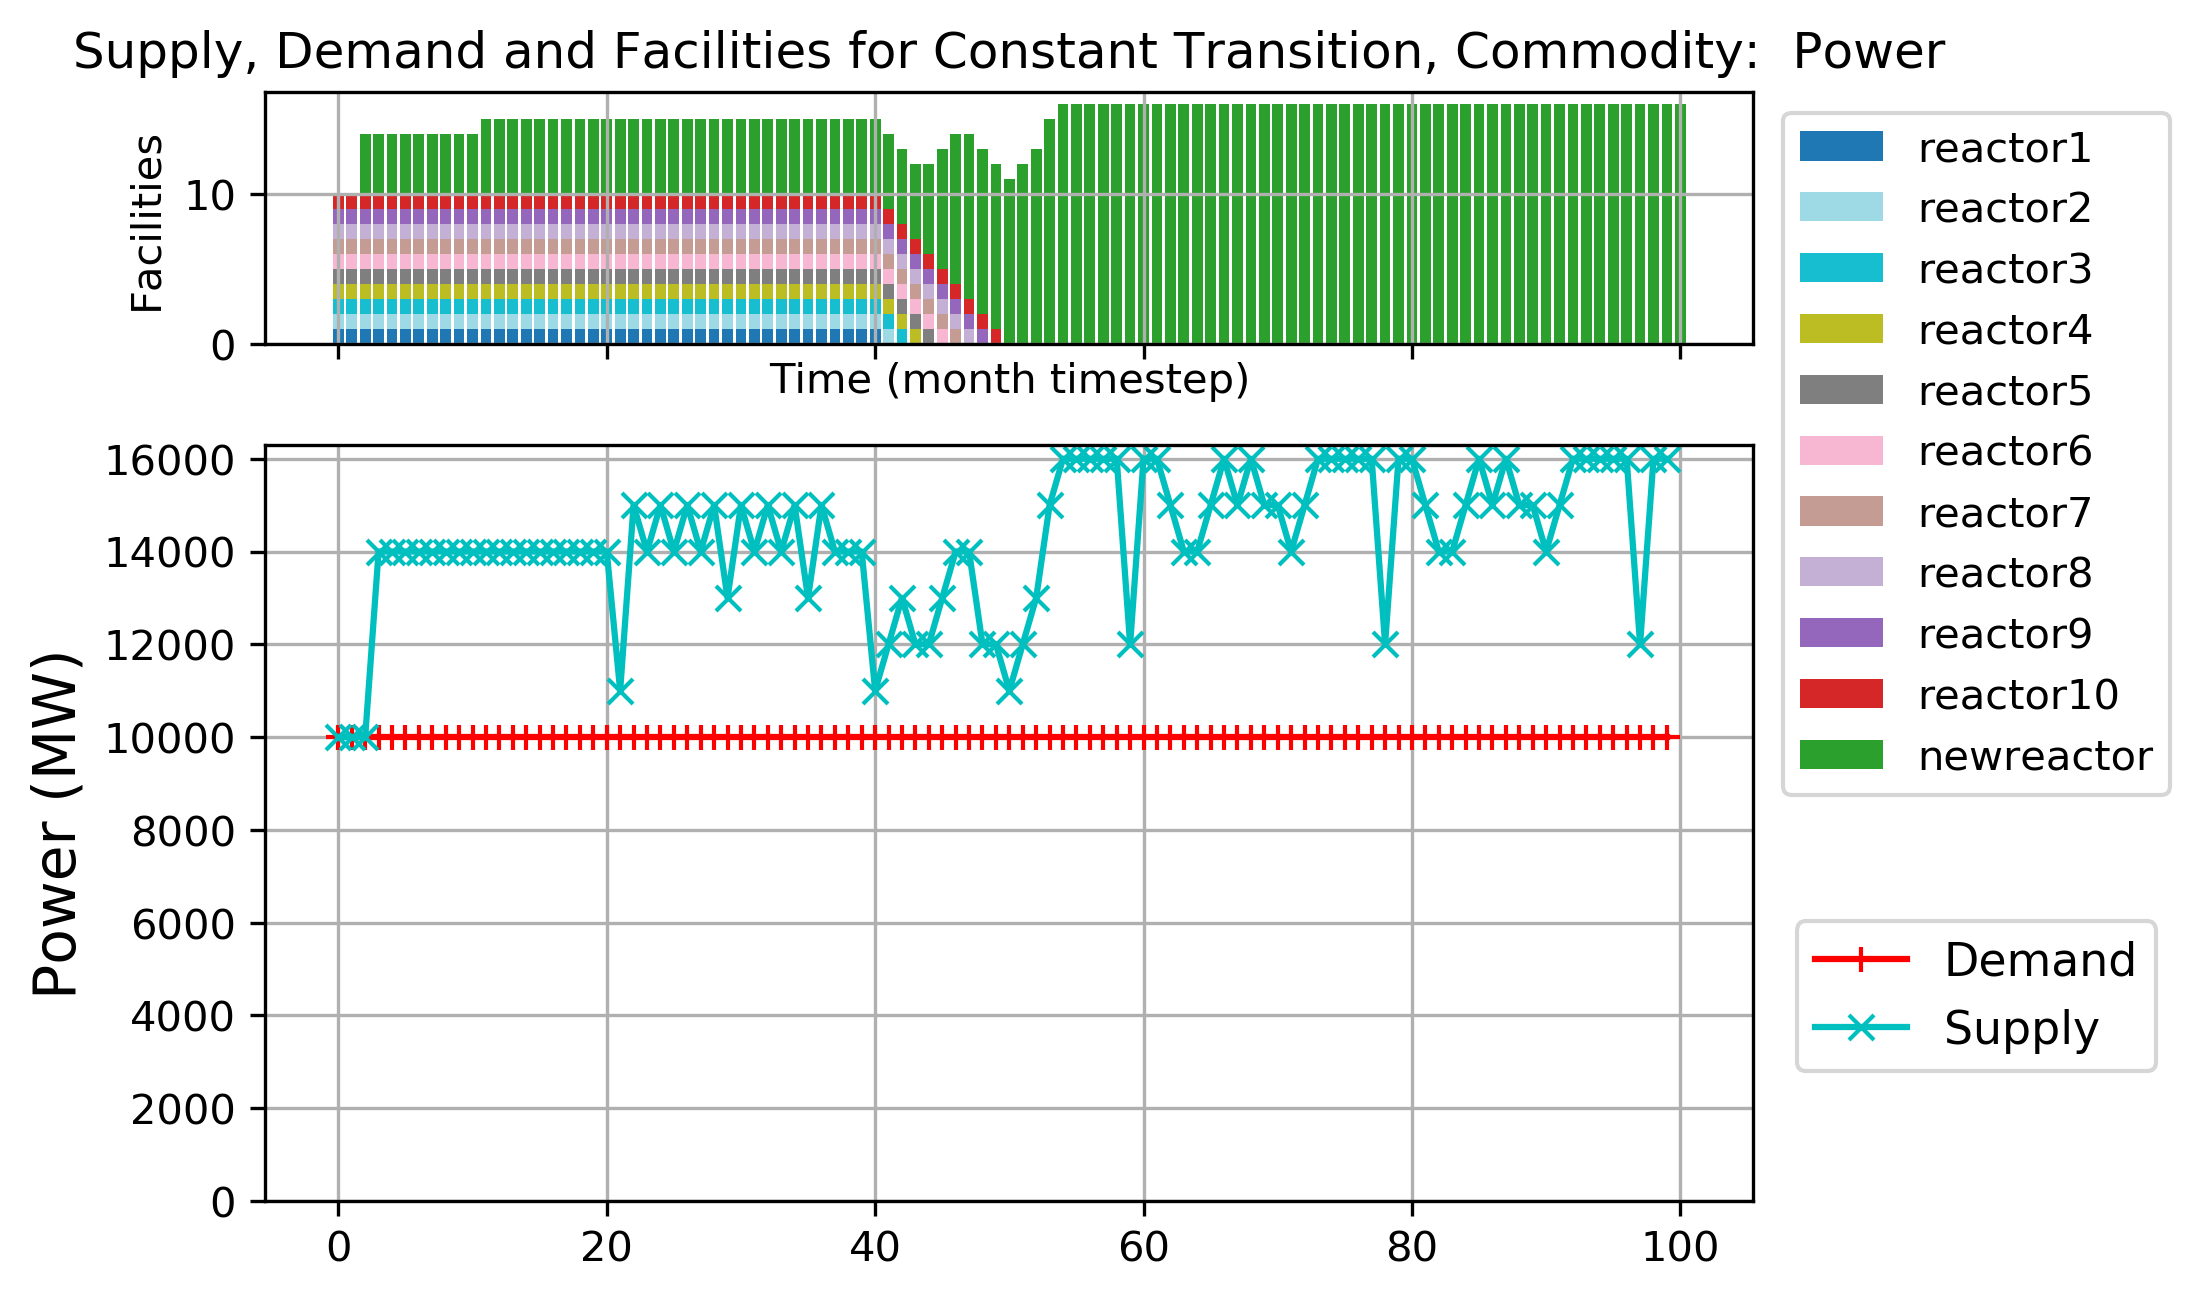
\includegraphics[width=0.9\linewidth]{figures/constanttransition-power.png} 
            \caption{Power demand and supply, and reactor facility deployment for  
            a simple constant power demand transition scenario with 
            three facility types: \texttt{source}, \texttt{reactor}, and \texttt{sink}.
            There are no time steps with power undersupply 
            \cite{chee_arfc/transition-scenarios_2018}.}
            \label{fig:constanttransition-power}
    \end{figure}

    \begin{figure}[]
        \centering
        \begin{subfigure}[t]{1\textwidth}
            \centering
            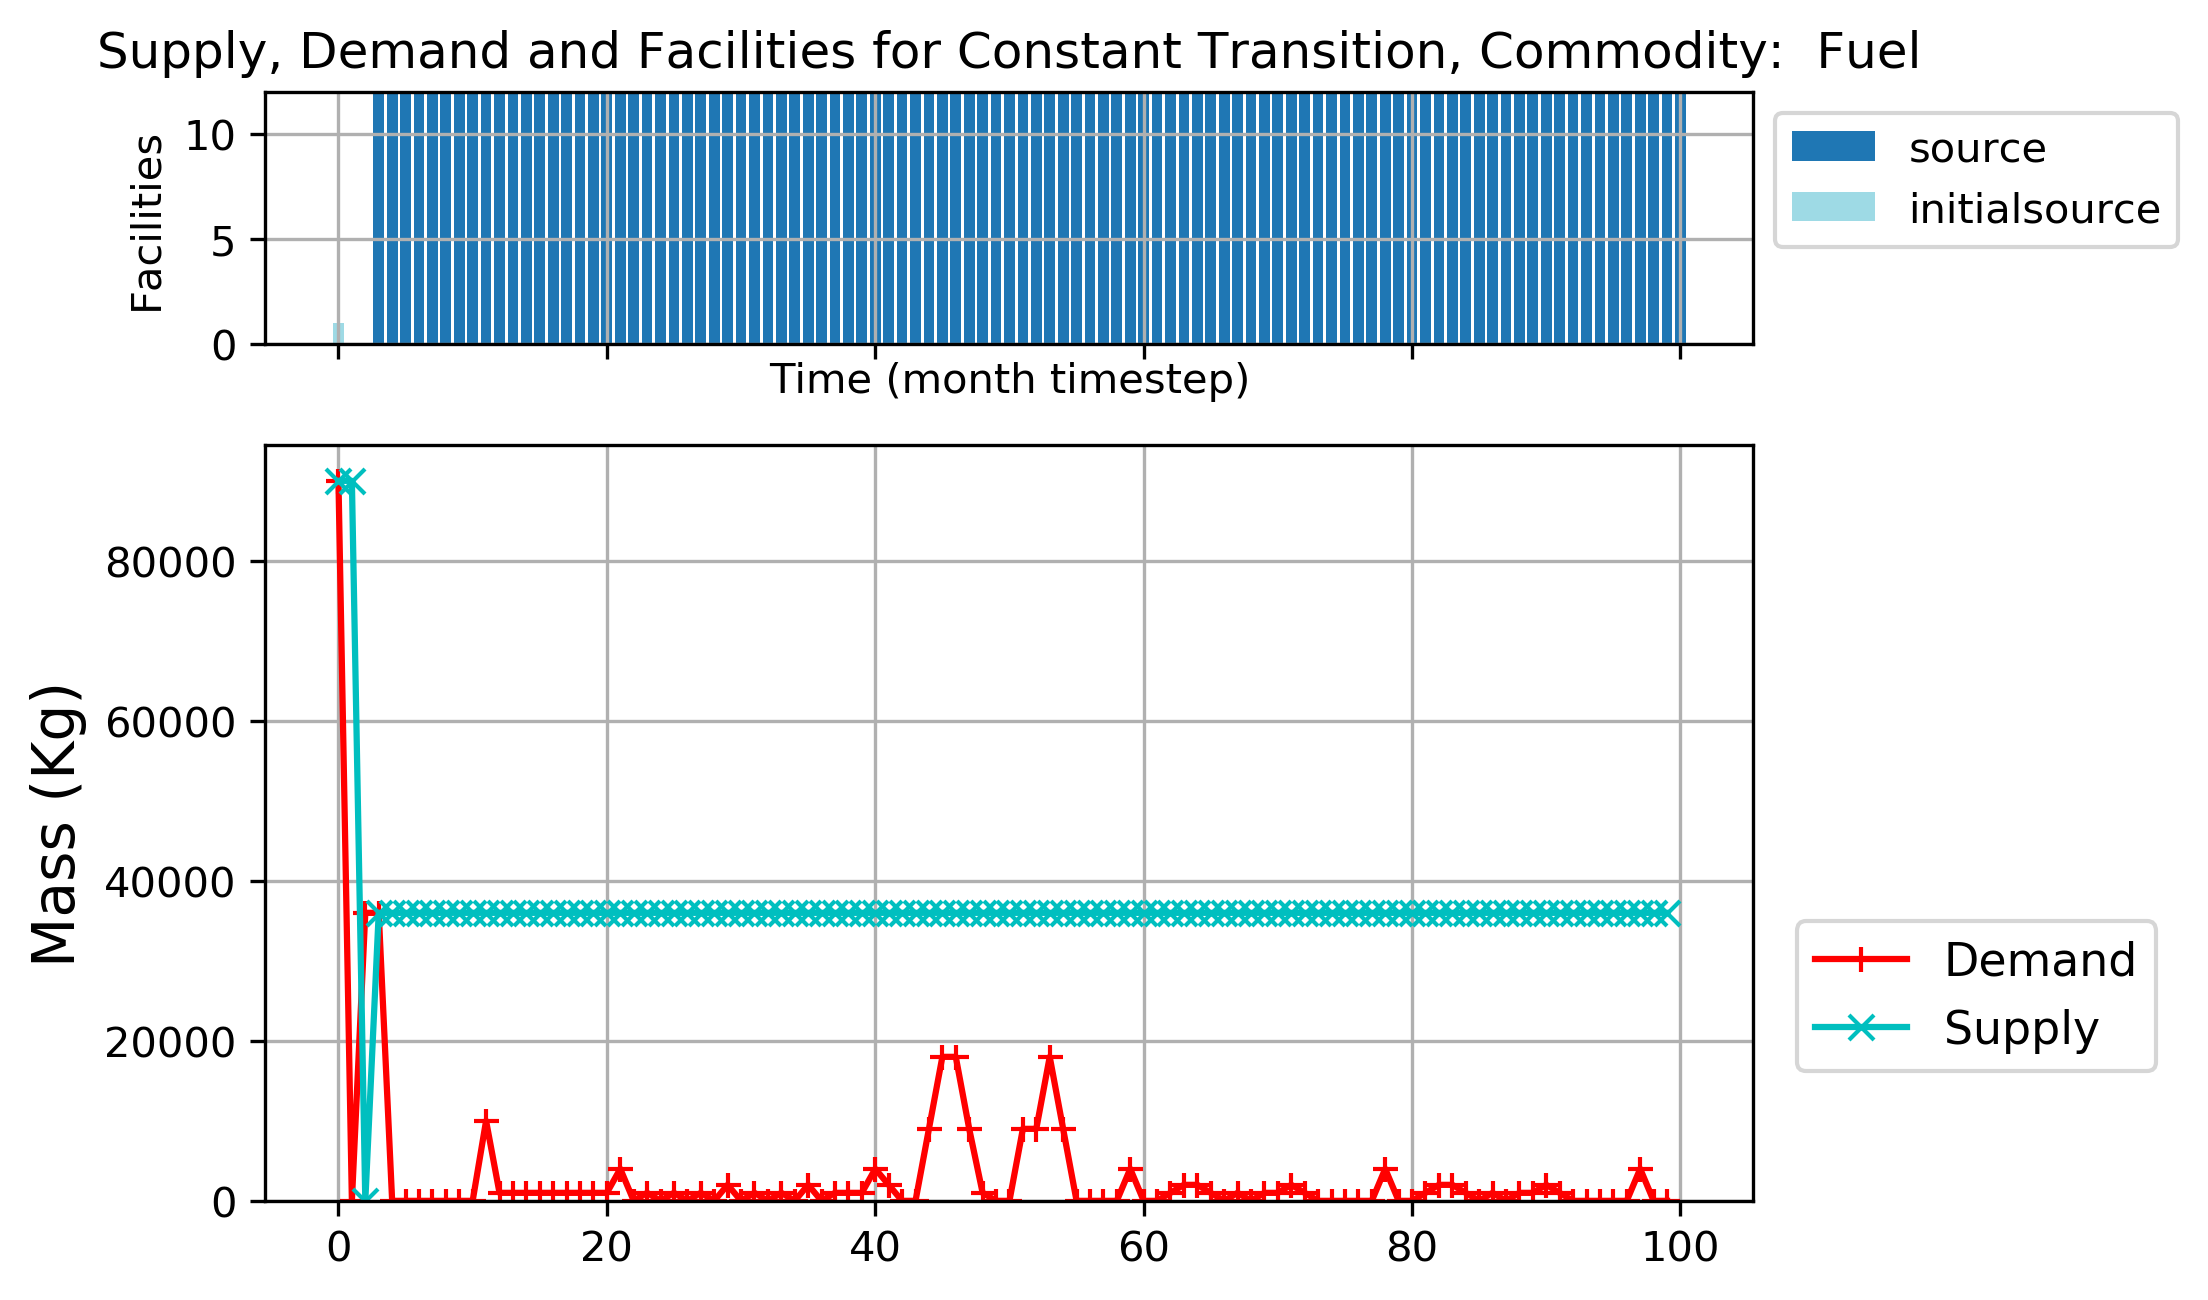
\includegraphics[width=0.9\linewidth]{figures/constanttransition-fuel.png} 
            \caption{Fuel demand and supply, and source facility deployment.
            Reactor facilities demand fuel and source facilities supply it.
            There is only one time step with fuel undersupply \cite{chee_arfc/transition-scenarios_2018}.}
            \label{fig:constanttransition-fuel}
        \end{subfigure}
        \begin{subfigure}[t]{1\textwidth}
            \centering
            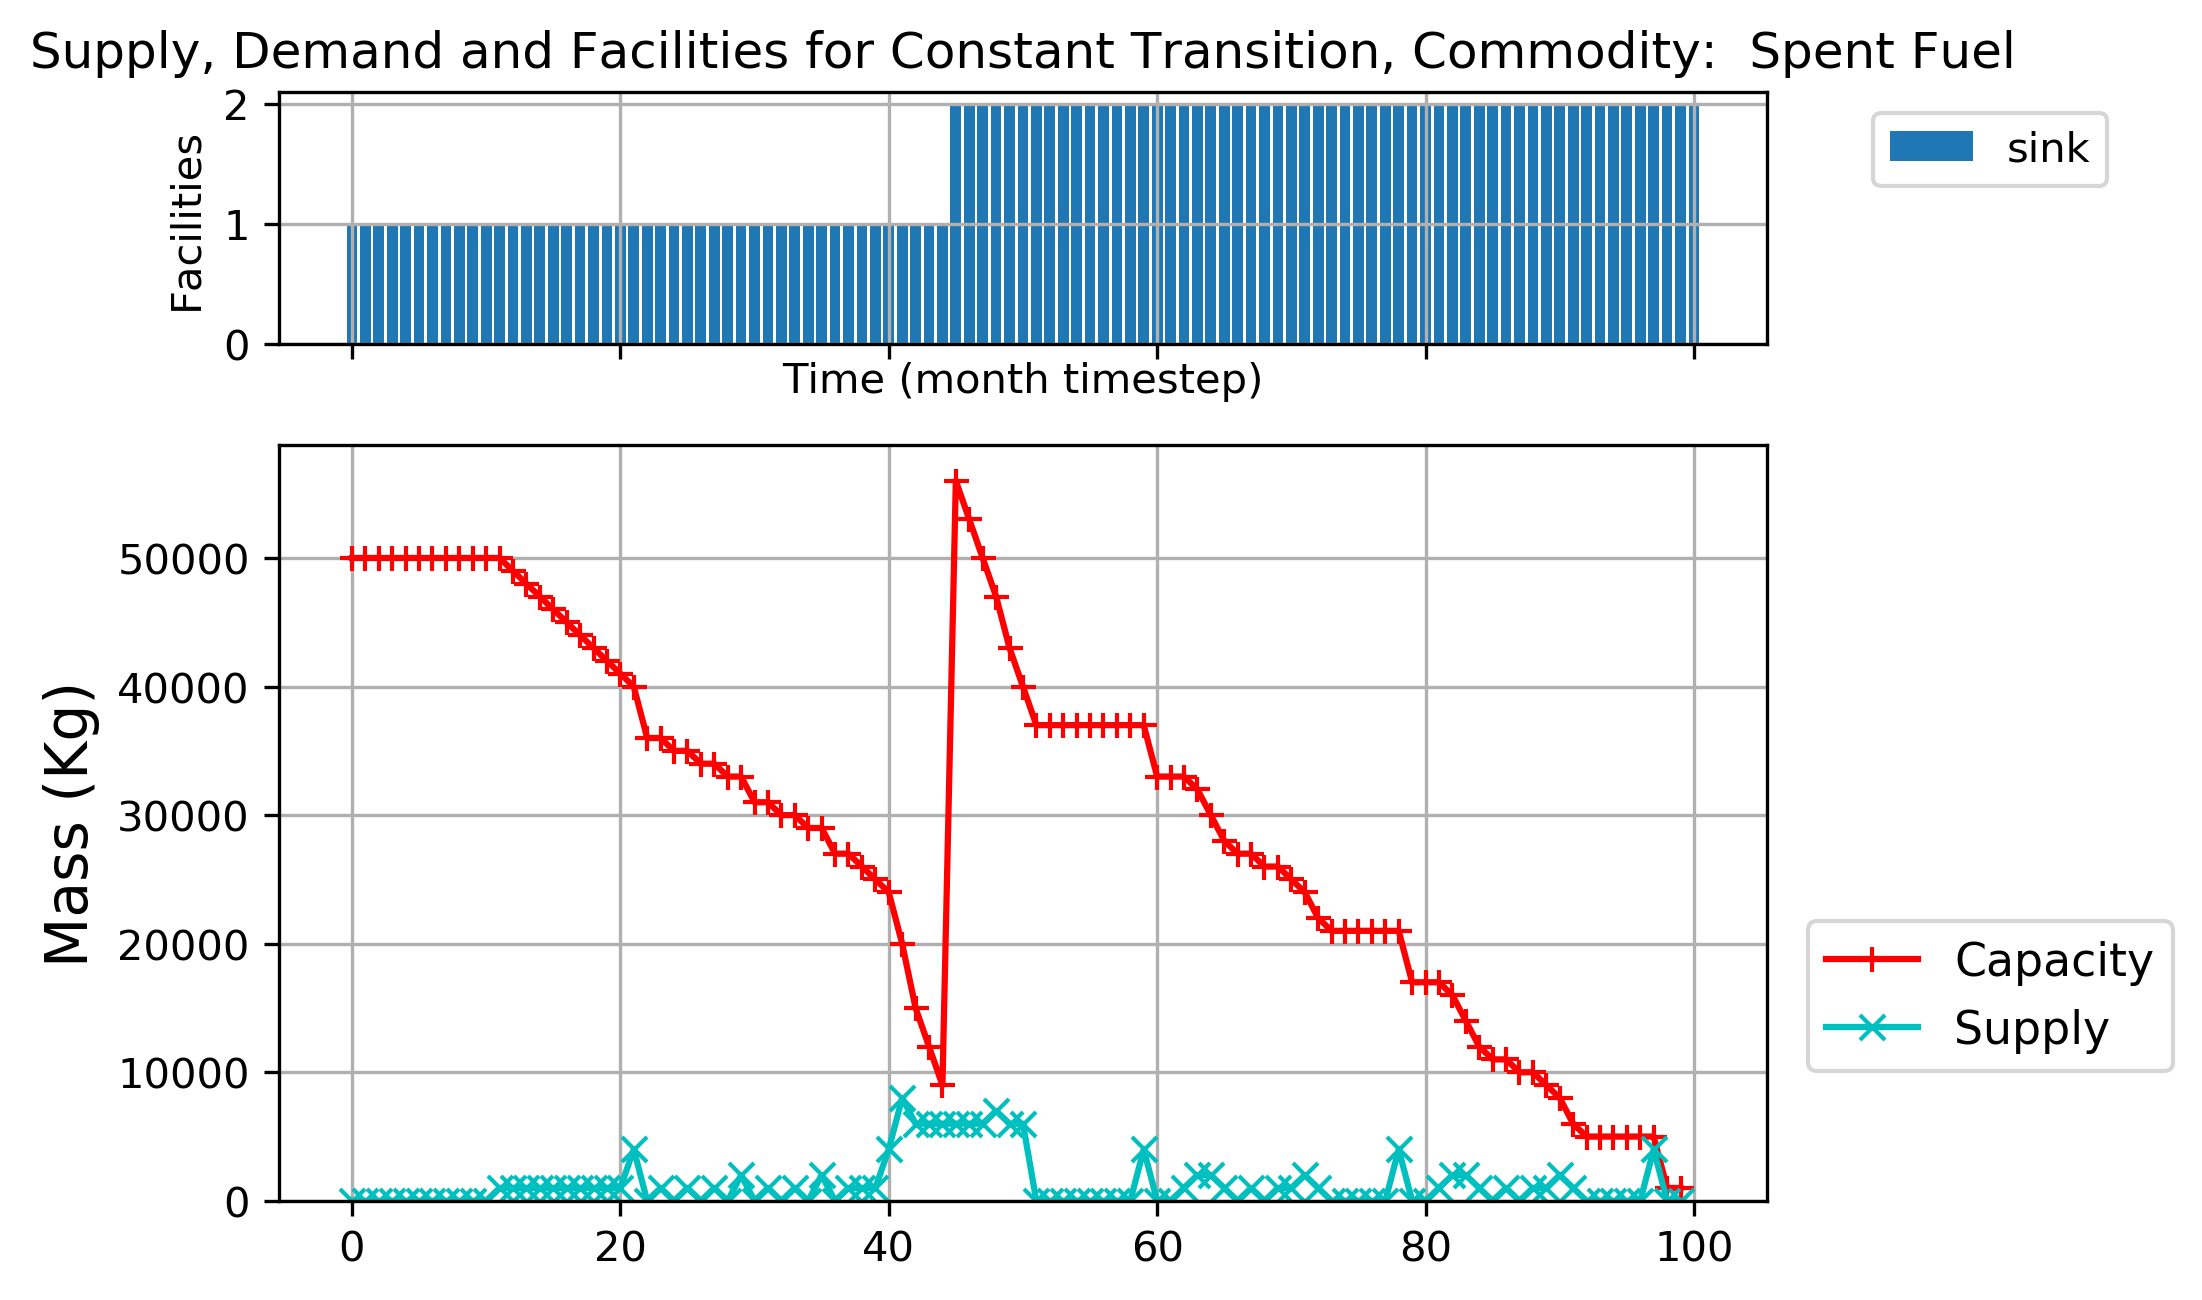
\includegraphics[width=0.9\linewidth]{figures/constanttransition-spentfuel.png} 
            \caption{Spent fuel demand and supply, and sink facility deployment.
                Spent fuel is supplied by reactors and the capacity to store them 
                is provided by sink facilities.
            There are no time steps with under-capacity of sink space \cite{chee_arfc/transition-scenarios_2018}.}
            \label{fig:constanttransition-spentfuel}
        \end{subfigure}
        \caption{Simple constant power demand transition scenario with 
        three facility types: \texttt{source}, \texttt{reactor}, and \texttt{sink}.}
    \end{figure}

    \subsection{Simple Transition Scenario Simulation: Linearly Increasing Demand}

    Figures \ref{fig:growingtransition-power}, \ref{fig:growingtransition-fuel},
    and \ref{fig:growingtransition-spentfuel} demonstrate \deploy's capability 
    to deploy reactors and supporting facilities to minimize undersupply 
    when meeting linearly increasing power demand and subsequent secondary 
    commodities demand. 
    This transition utilizes a smaller power supply buffer compared with the constant 
    power transition scenario.
    Table \ref{tab:transition-scenario-results} shows the number of 
    undersupplied timesteps. 
    In Figure \ref{fig:growingtransition-power}, there is no power supply gaps, demonstrating that 
    \deploy successfully deployed \texttt{source} \texttt{reactor}, and \texttt{sink} 
    facilities to create the supply chain to meet the linearly-increasing power demand. 
    \begin{figure}[]
        \centering
        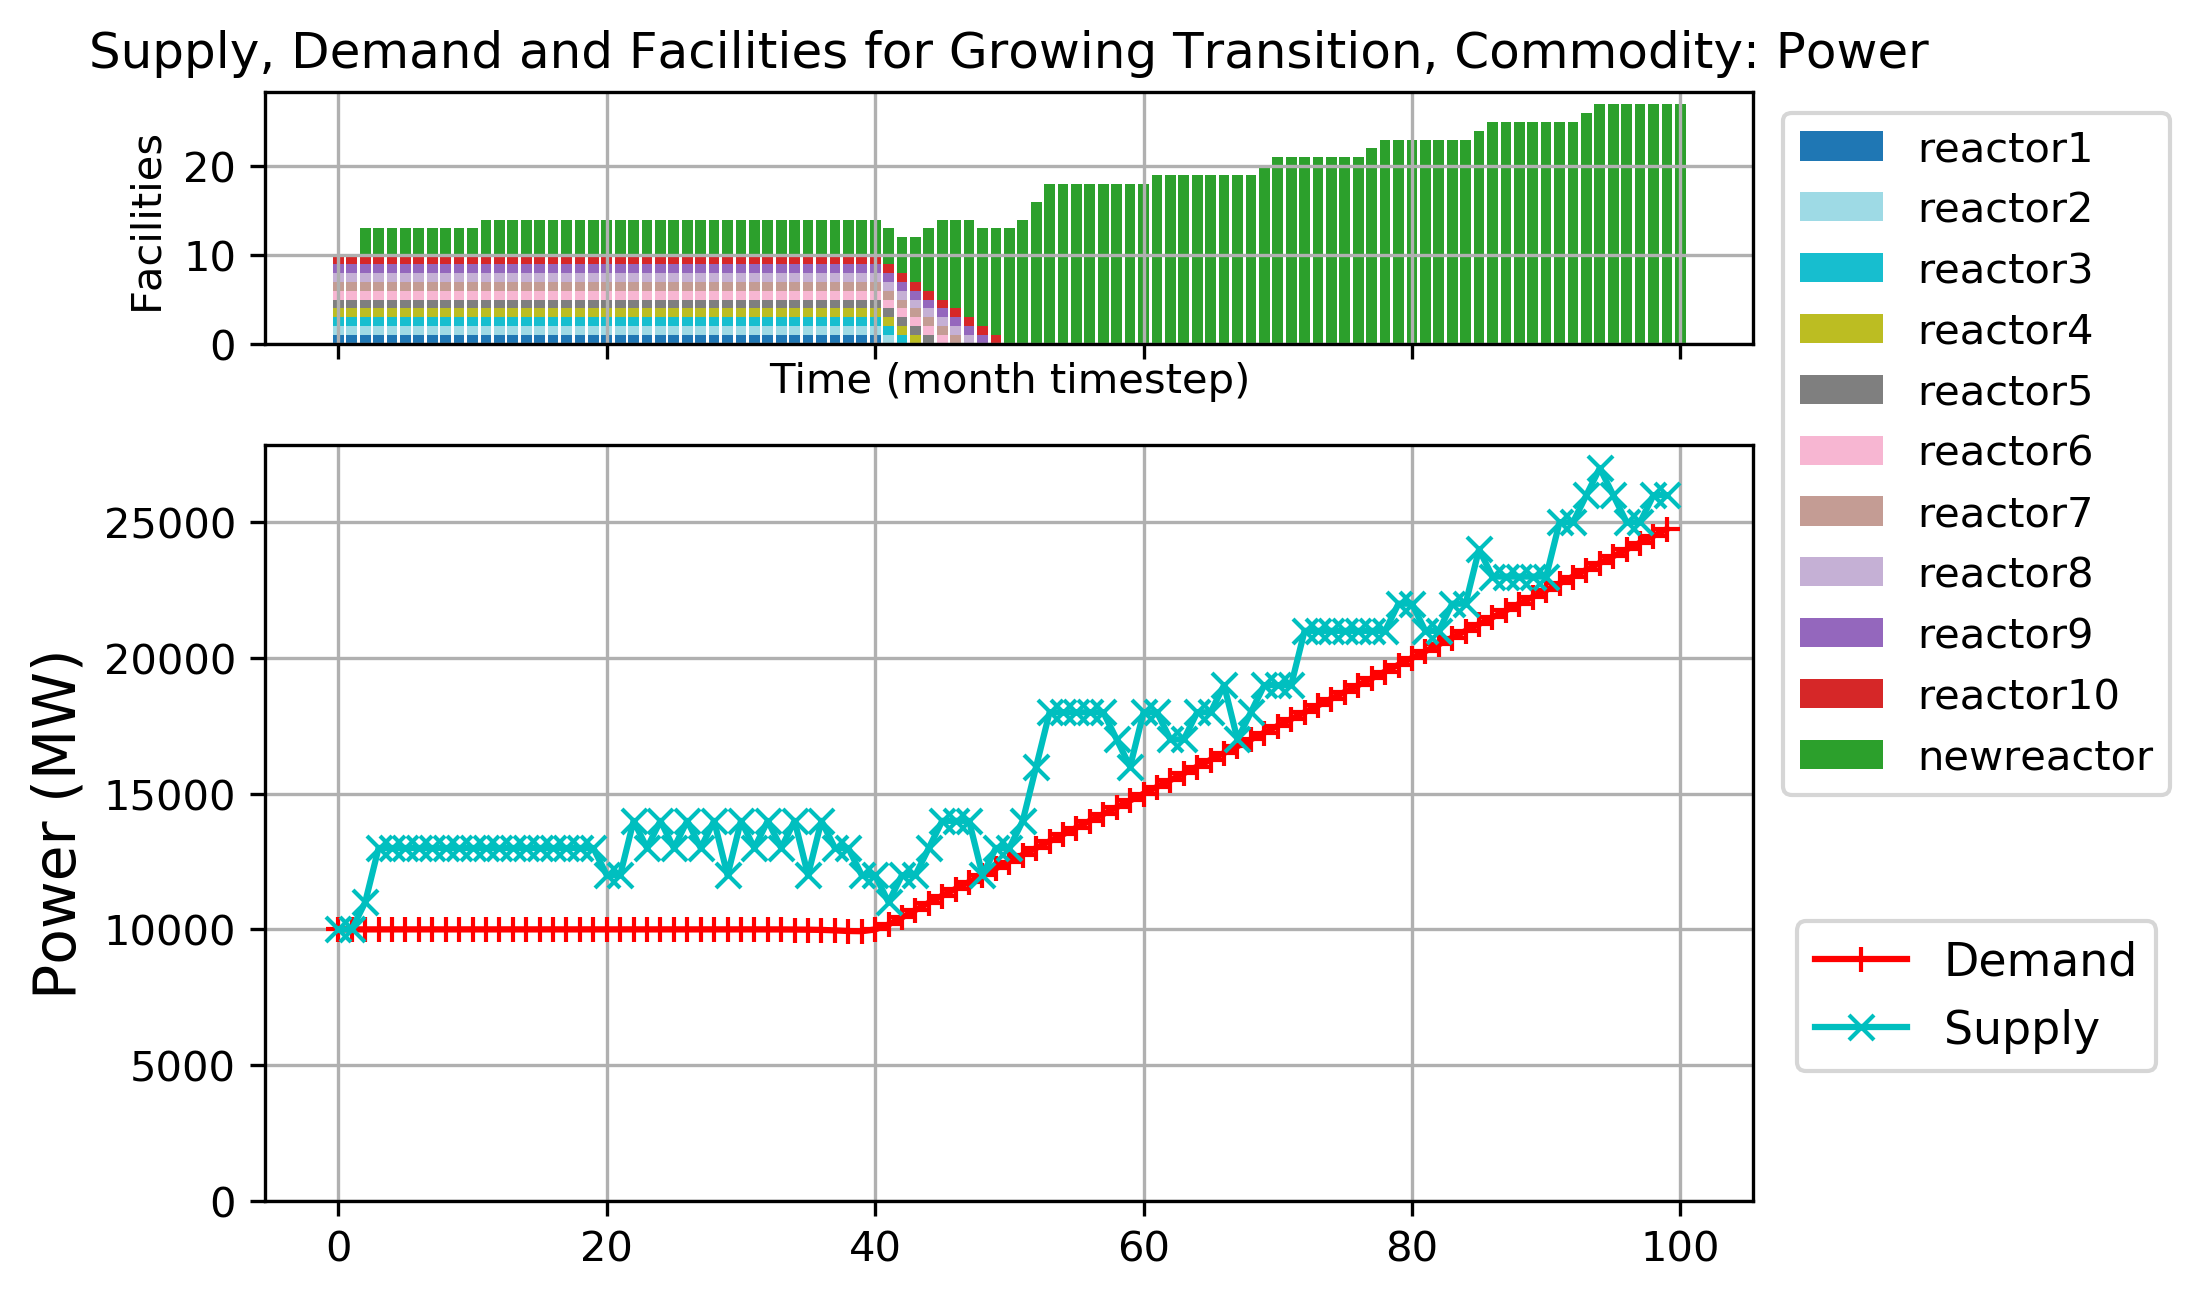
\includegraphics[width=0.9\linewidth]{figures/growingtransition-power.png} 
            \caption{Power demand and supply, and reactor facility deployment plot for  
            a simple linearly increasing power demand transition scenario with 
            three facility types: \texttt{source}, \texttt{reactor}, and \texttt{sink}.
            There are no time steps with power undersupply\cite{chee_arfc/transition-scenarios_2018}.}
            \label{fig:growingtransition-power}
    \end{figure}
    
    \begin{figure}[]
        \centering
        \begin{subfigure}[t]{\textwidth}
            \centering
            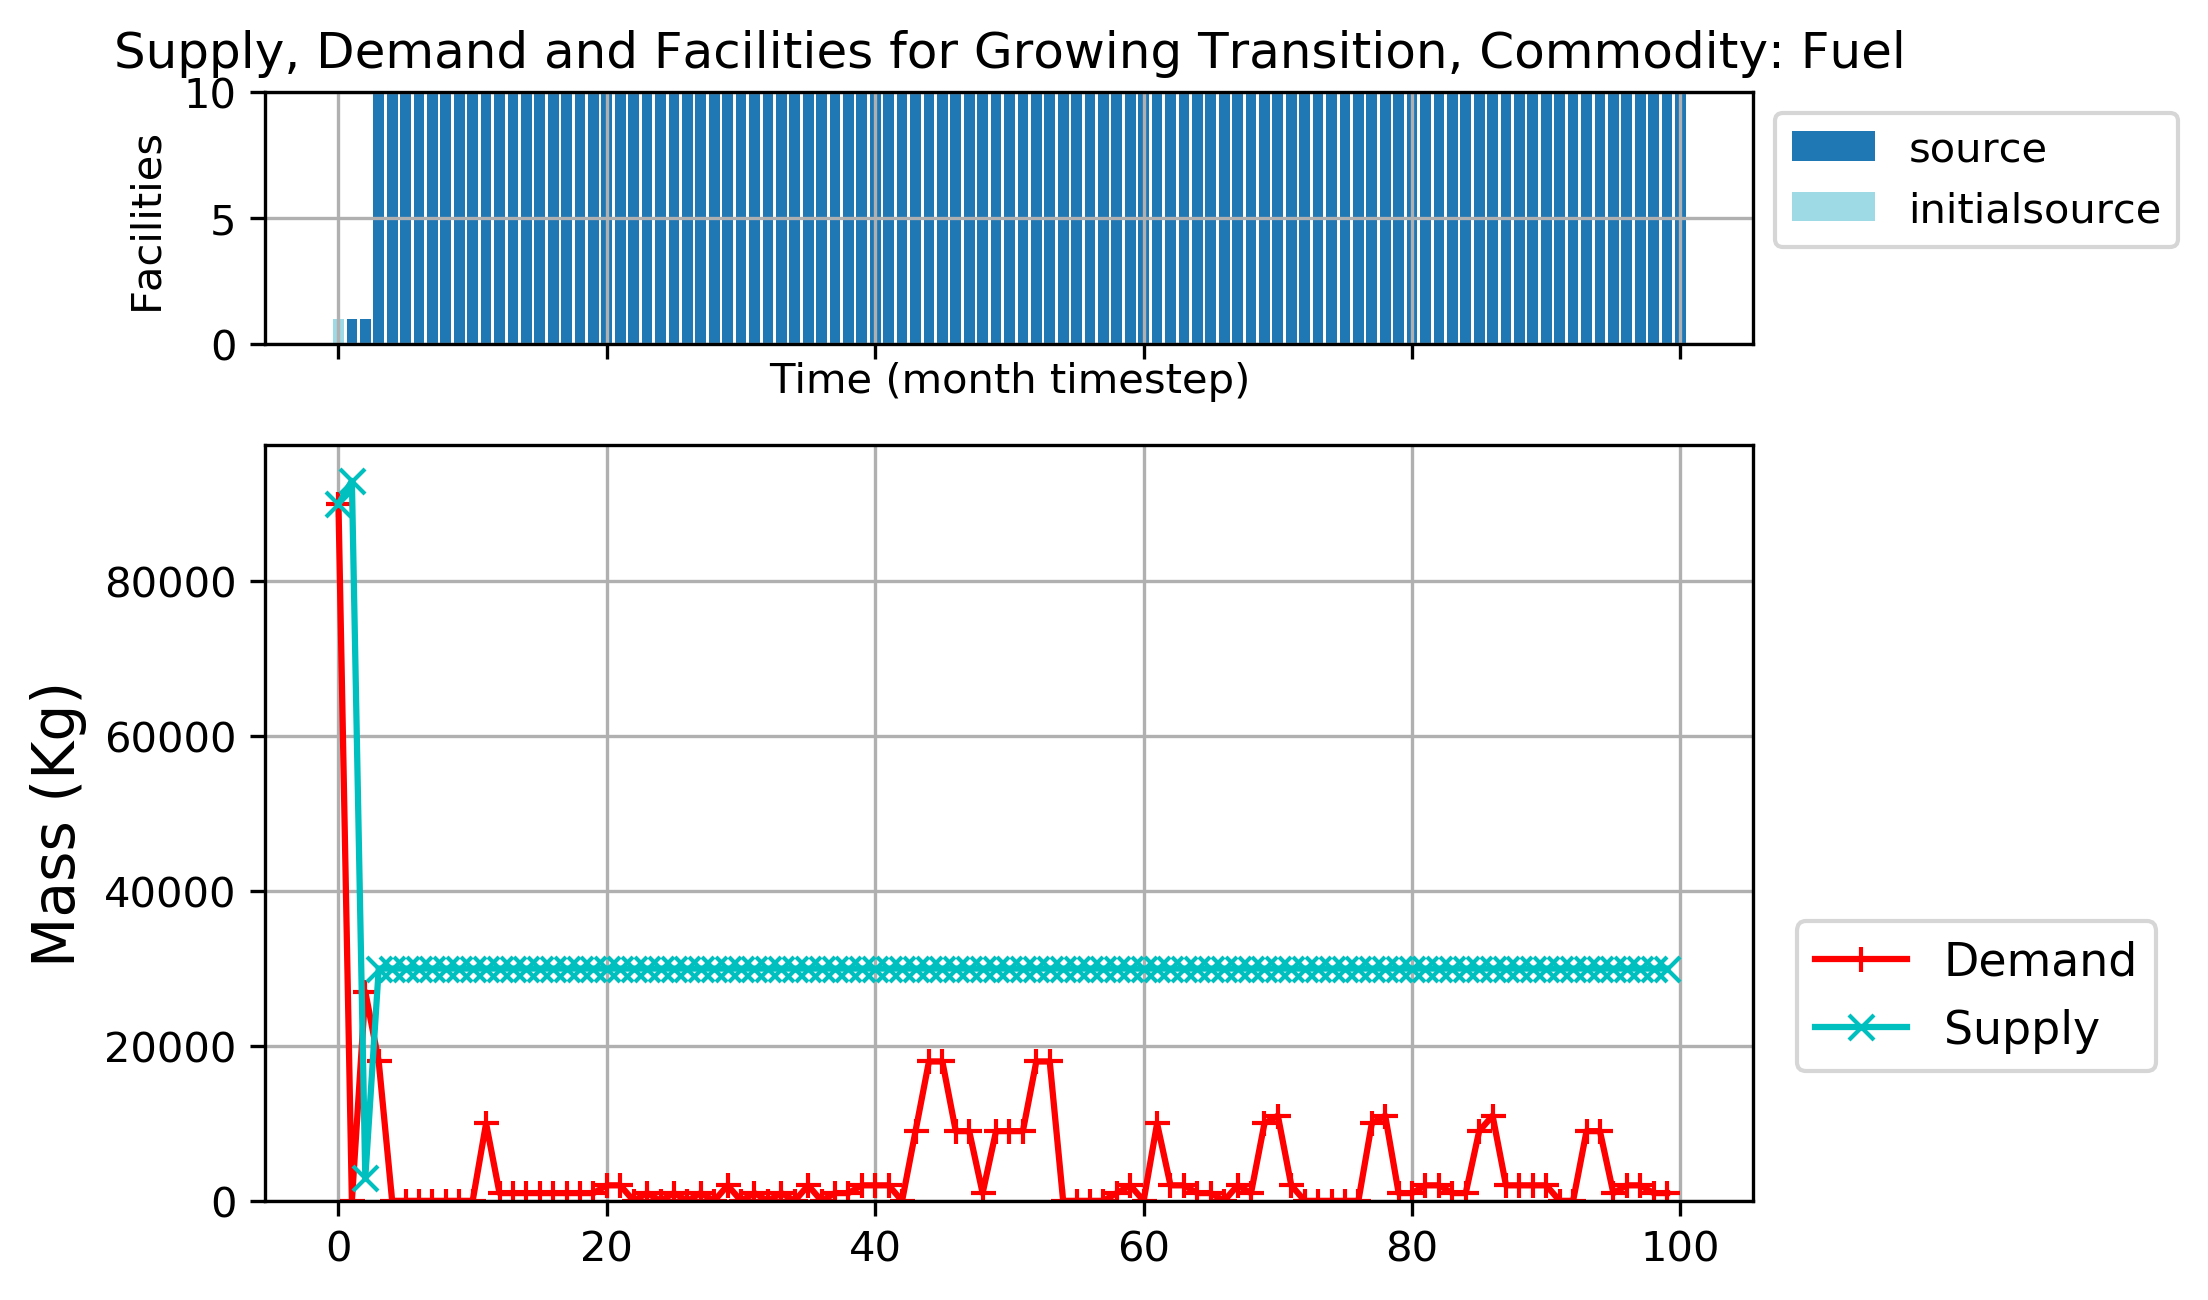
\includegraphics[width=0.9\linewidth]{figures/growingtransition-fuel.png} 
            \caption{Fuel demand and supply, and source facility deployment plot.
            Reactor facilities demand fuel and source facilities supply it.
            There is only one time step with fuel undersupply \cite{chee_arfc/transition-scenarios_2018}.}
            \label{fig:growingtransition-fuel}
        \end{subfigure}
        \begin{subfigure}[t]{\textwidth}
            \centering
            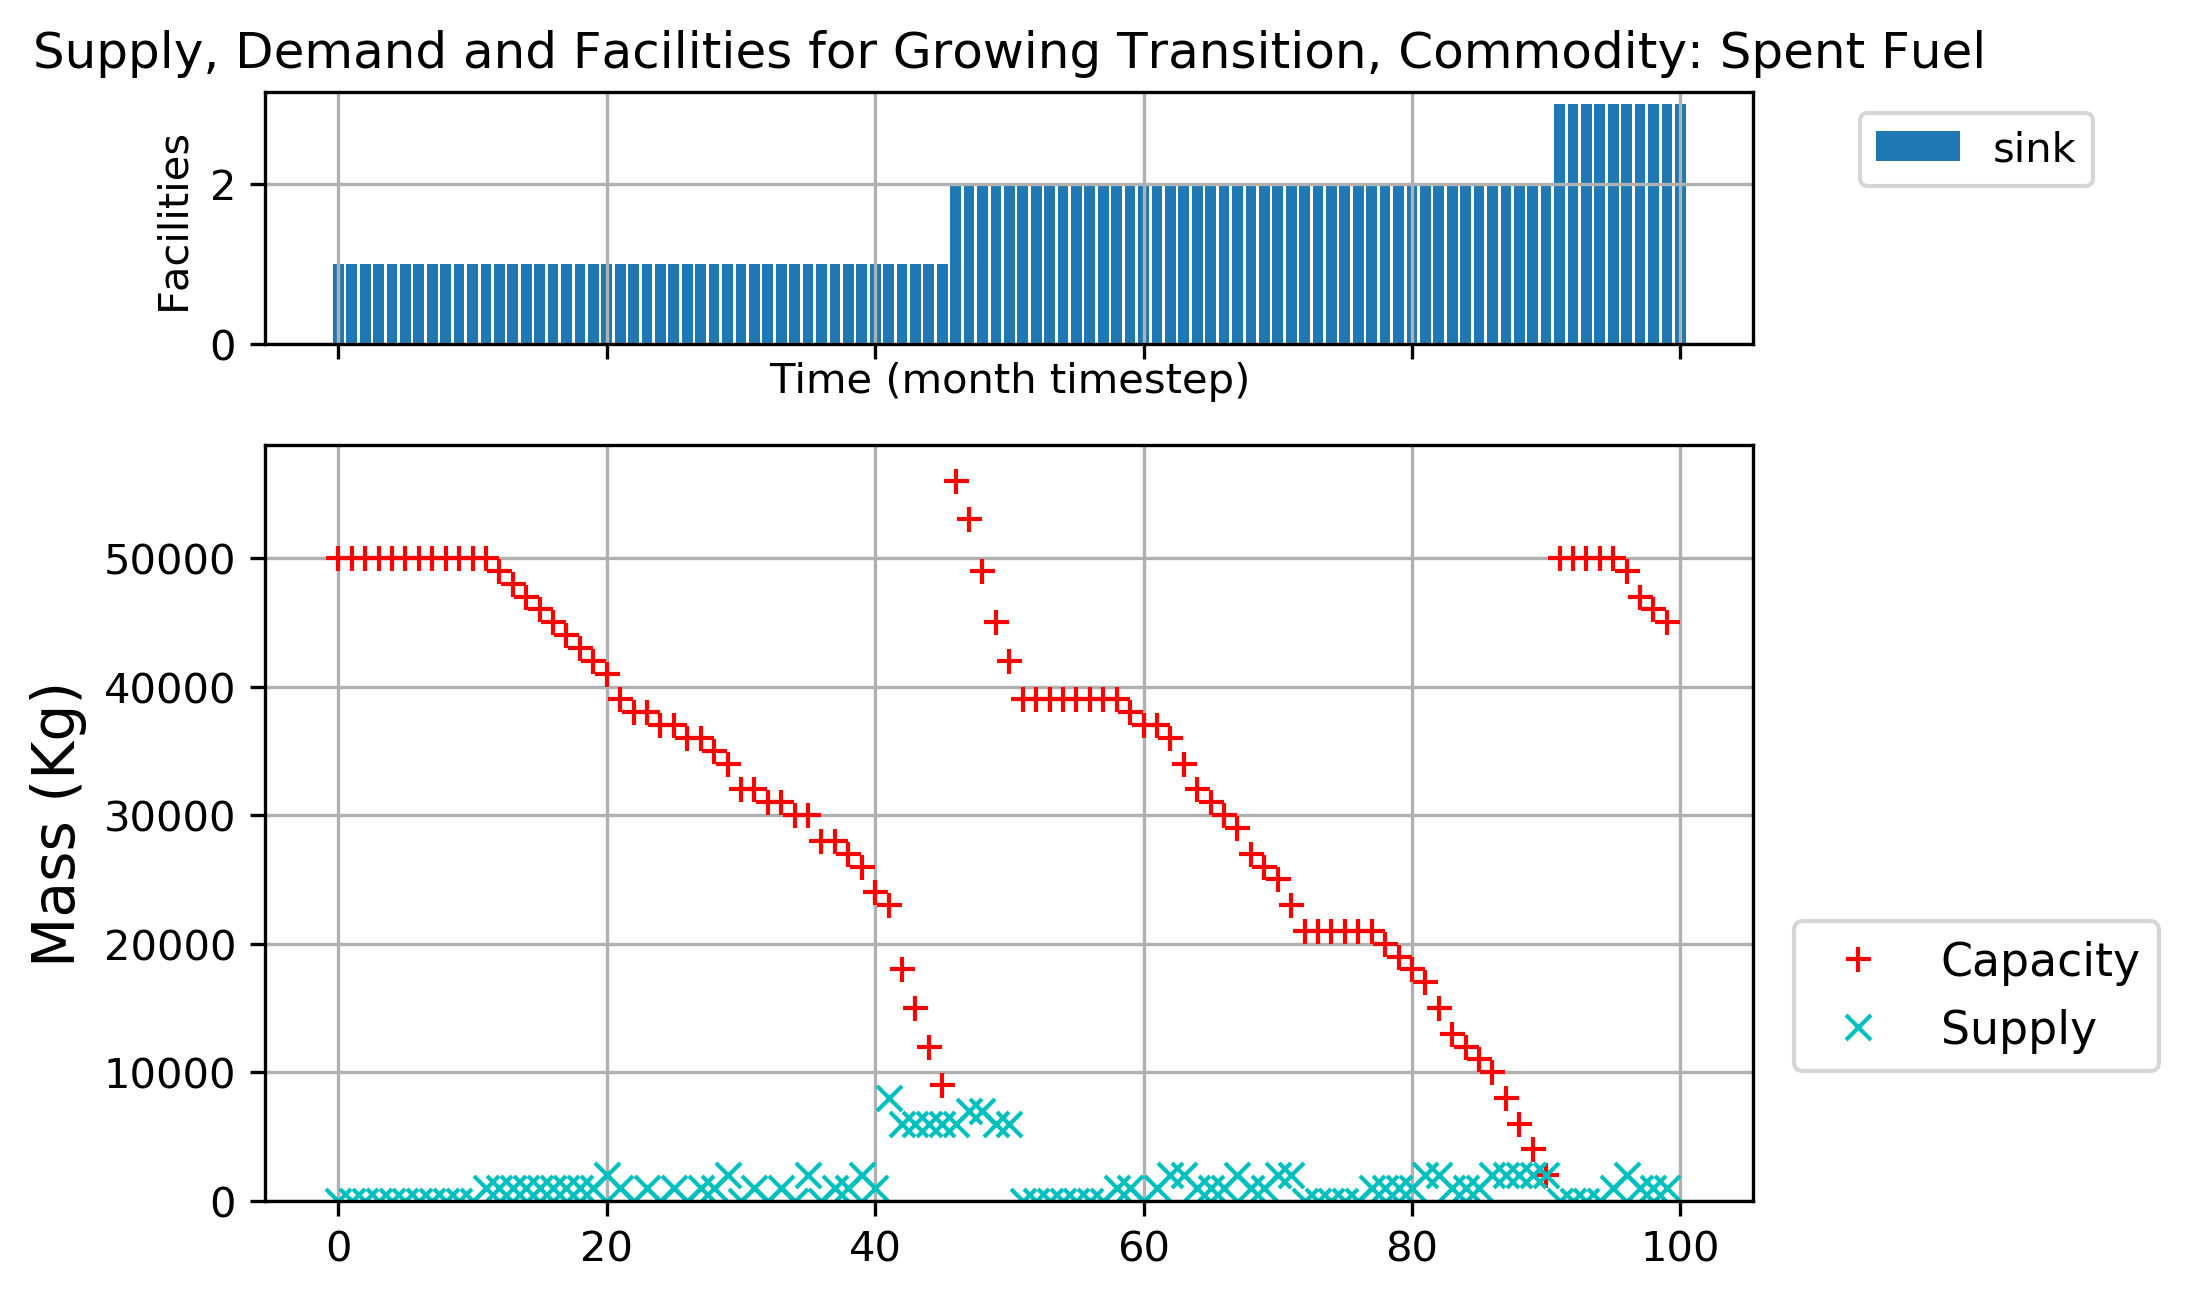
\includegraphics[width=0.9\linewidth]{figures/growingtransition-spentfuel.png} 
            \caption{Spent fuel demand and supply, and sink facility deployment plot.
                Spent fuel is supplied by reactors and the capacity to store them 
                is provided by sink facilities.
            There are no time steps with under-capacity of sink space \cite{chee_arfc/transition-scenarios_2018}.}
            \label{fig:growingtransition-spentfuel}
        \end{subfigure}
        \caption{Simple linearly increasing power demand transition scenario with 
        three facility types: \texttt{source}, \texttt{reactor}, and \texttt{sink}.}
    \end{figure}
    
    \subsection{Simple Transition Scenario Simulation: Sinusoidal Demand}
    Real world power demand varies seasonally. 
    Accordingly, a sinusoidal power demand with a period of 6 month best 
    reflects reality. 
    Figures \ref{fig:sinetransition-power}, \ref{fig:sinetransition-fuel},
    and \ref{fig:sinetransition-spentfuel} demonstrate \deploy's capability 
    to deploy reactor and supporting facilities to meet a sinusoidal power
    demand. 
    Table \ref{tab:transition-scenario-results} shows the number of 
    undersupplied timesteps.
    The \texttt{holt-winters} prediction method best minimizes power 
    undersupply.  
    This is because the \texttt{holt-winters} method excels in
    forecasting for repetitive seasonal time series data. 

    \begin{figure}[]
        \centering
        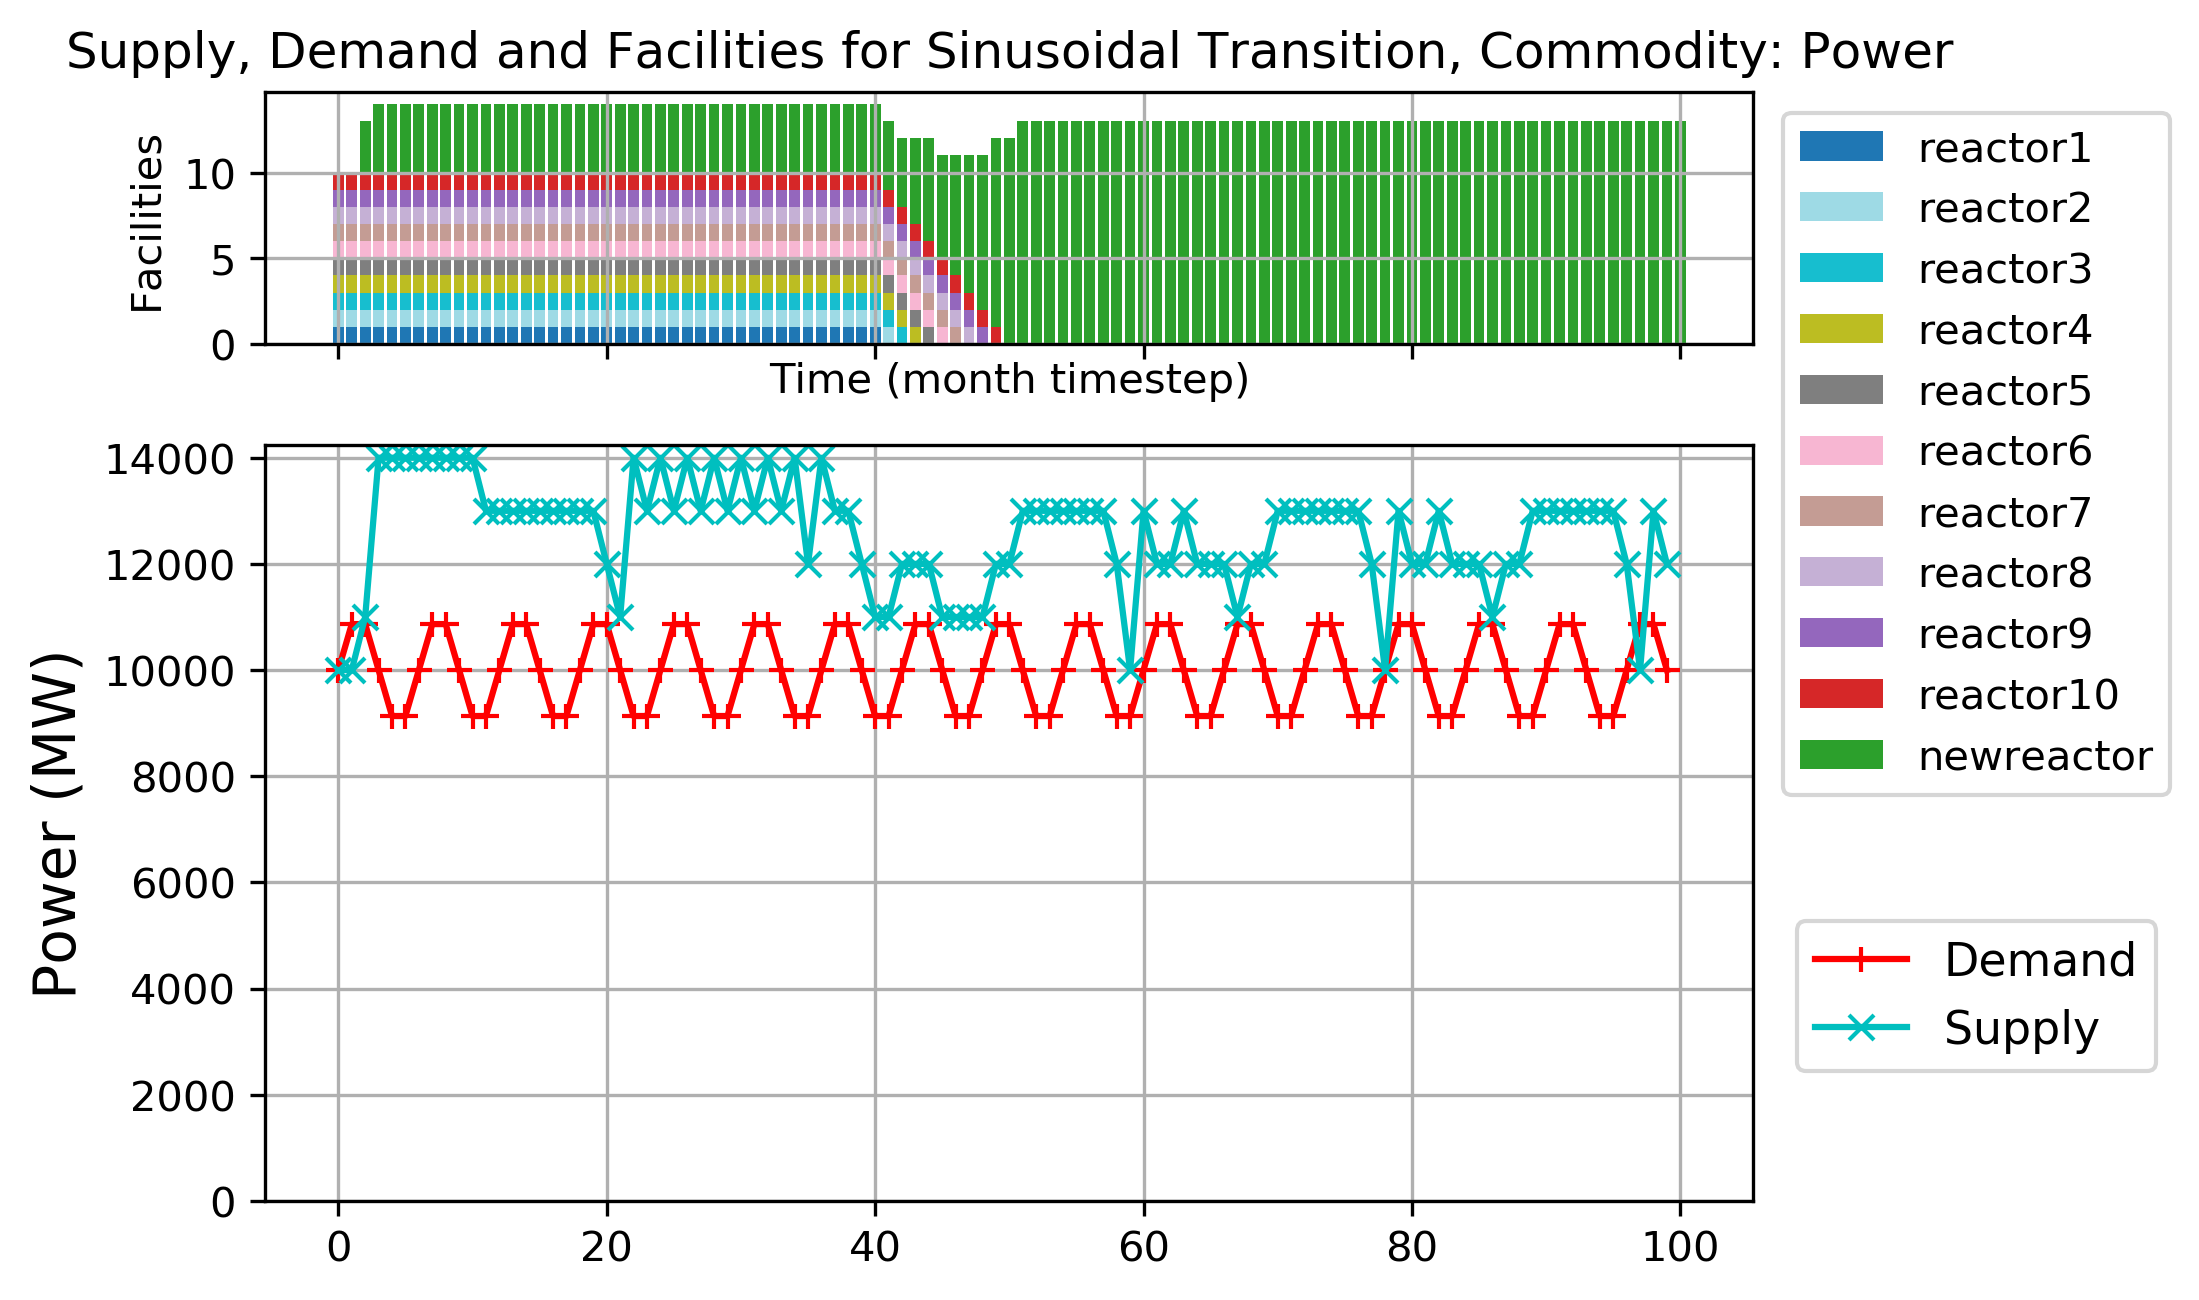
\includegraphics[width=0.9\linewidth]{figures/sinetransition-power.png} 
            \caption{Power demand and supply, and reactor facility deployment plot for  
            a simple sinusoidal power demand transition scenario with 
            three facility types: \texttt{source}, \texttt{reactor}, and \texttt{sink}.
            There are no time steps with power undersupply \cite{chee_arfc/transition-scenarios_2018}.}
            \label{fig:sinetransition-power}
    \end{figure}
    
    \begin{figure}[]
        \centering
        \begin{subfigure}[t]{\textwidth}
            \centering
            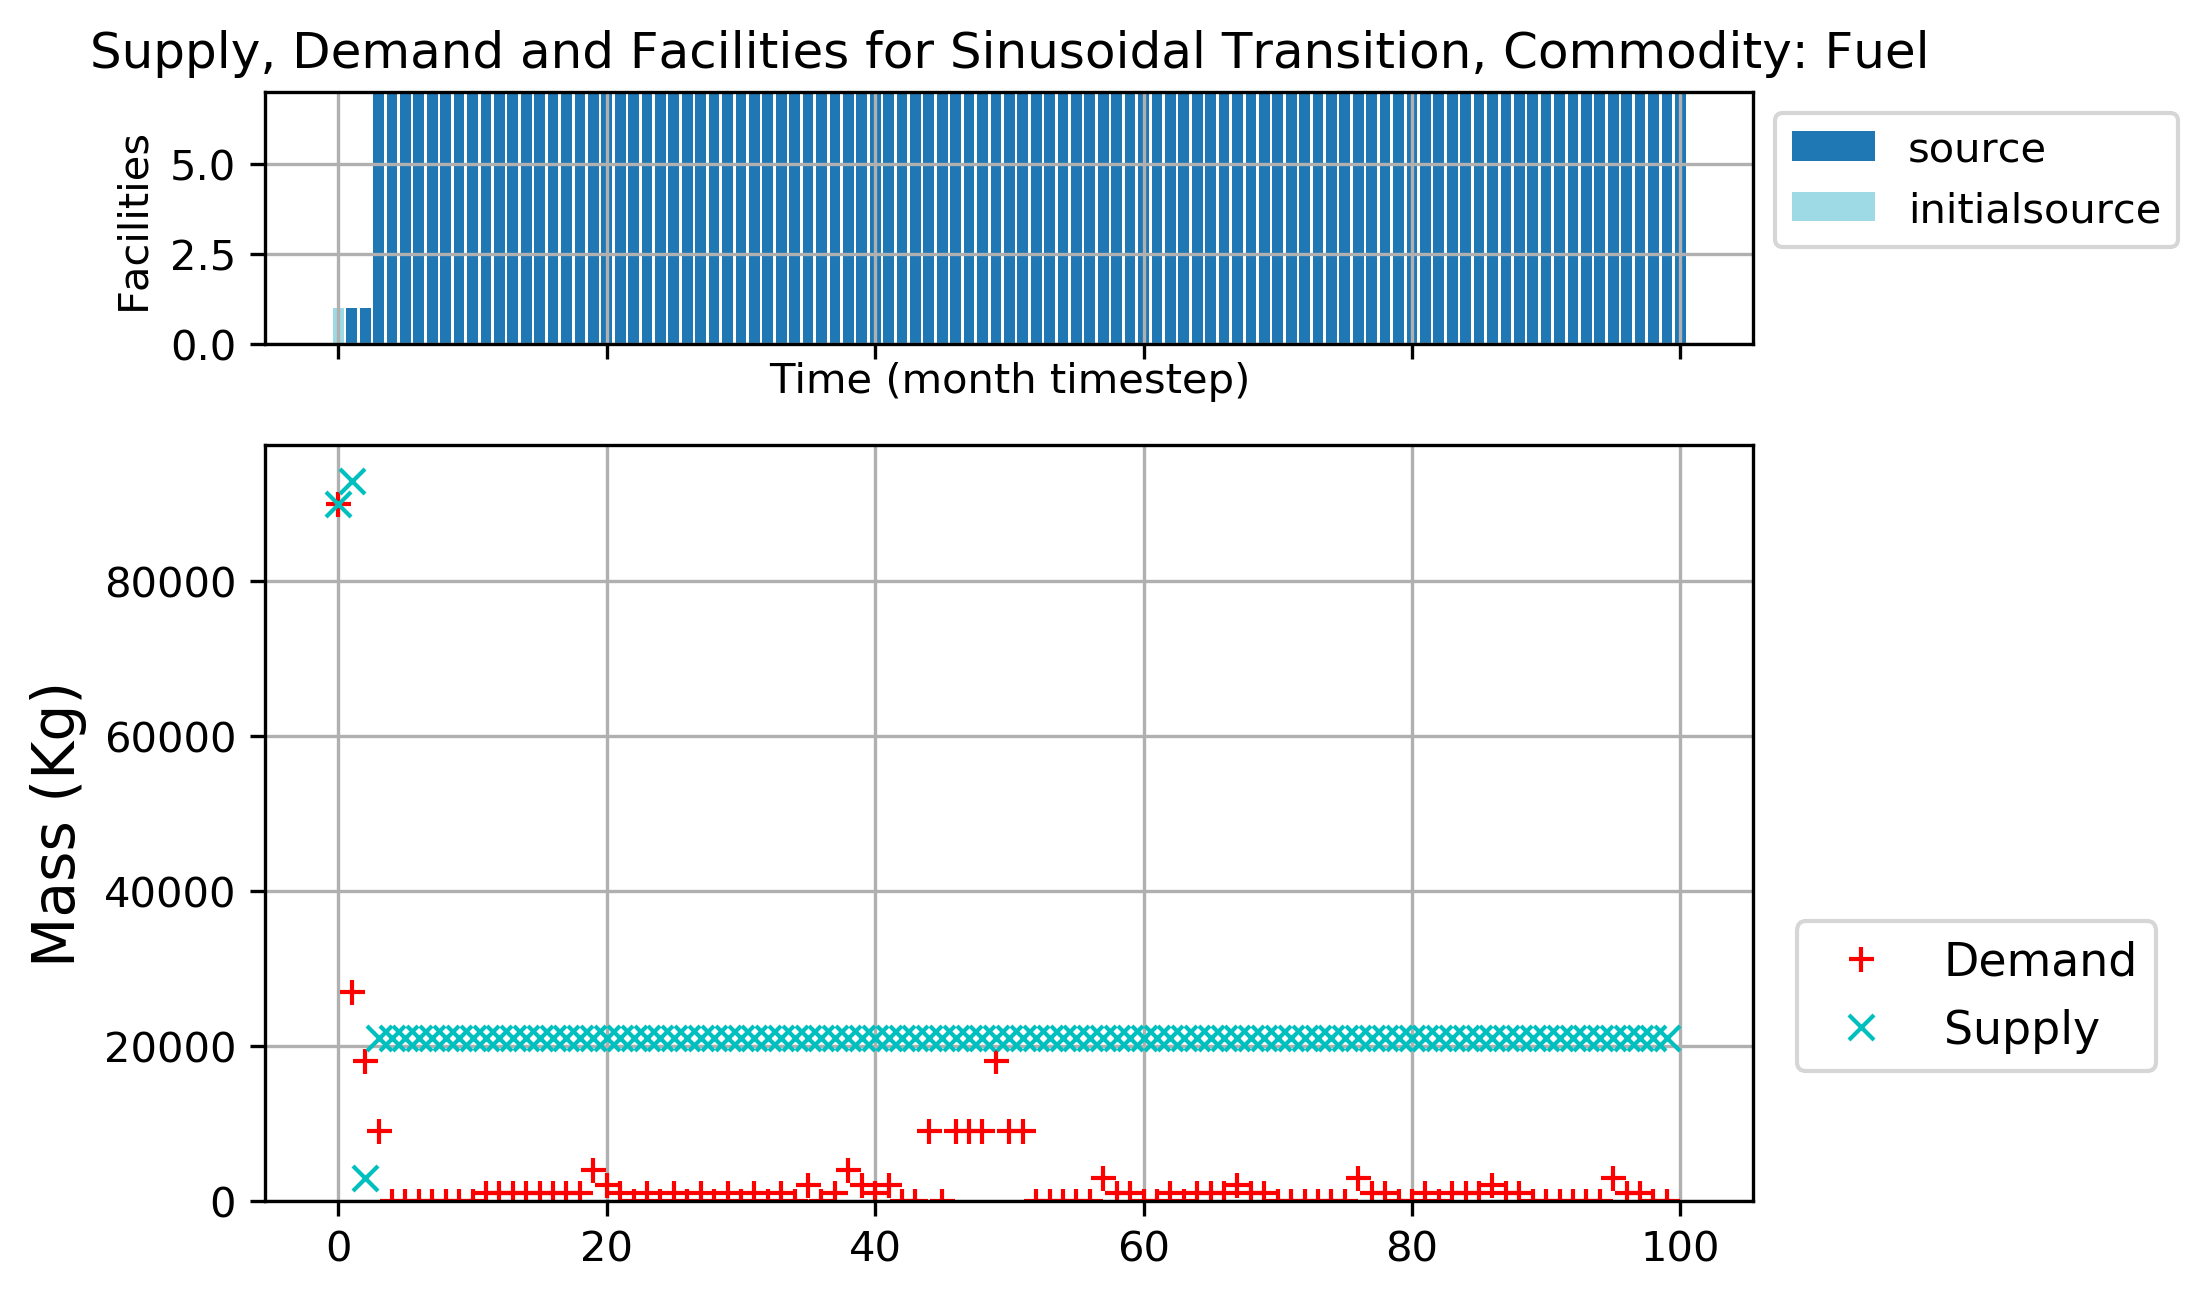
\includegraphics[width=0.9\linewidth]{figures/sinetransition-fuel.png} 
            \caption{Fuel demand and supply, and source facility deployment plot.
            Reactor facilities demand fuel and source facilities supply it.
            There is only one time step with fuel undersupply \cite{chee_arfc/transition-scenarios_2018}.}
            \label{fig:sinetransition-fuel}
        \end{subfigure}
        \begin{subfigure}[t]{\textwidth}
            \centering
            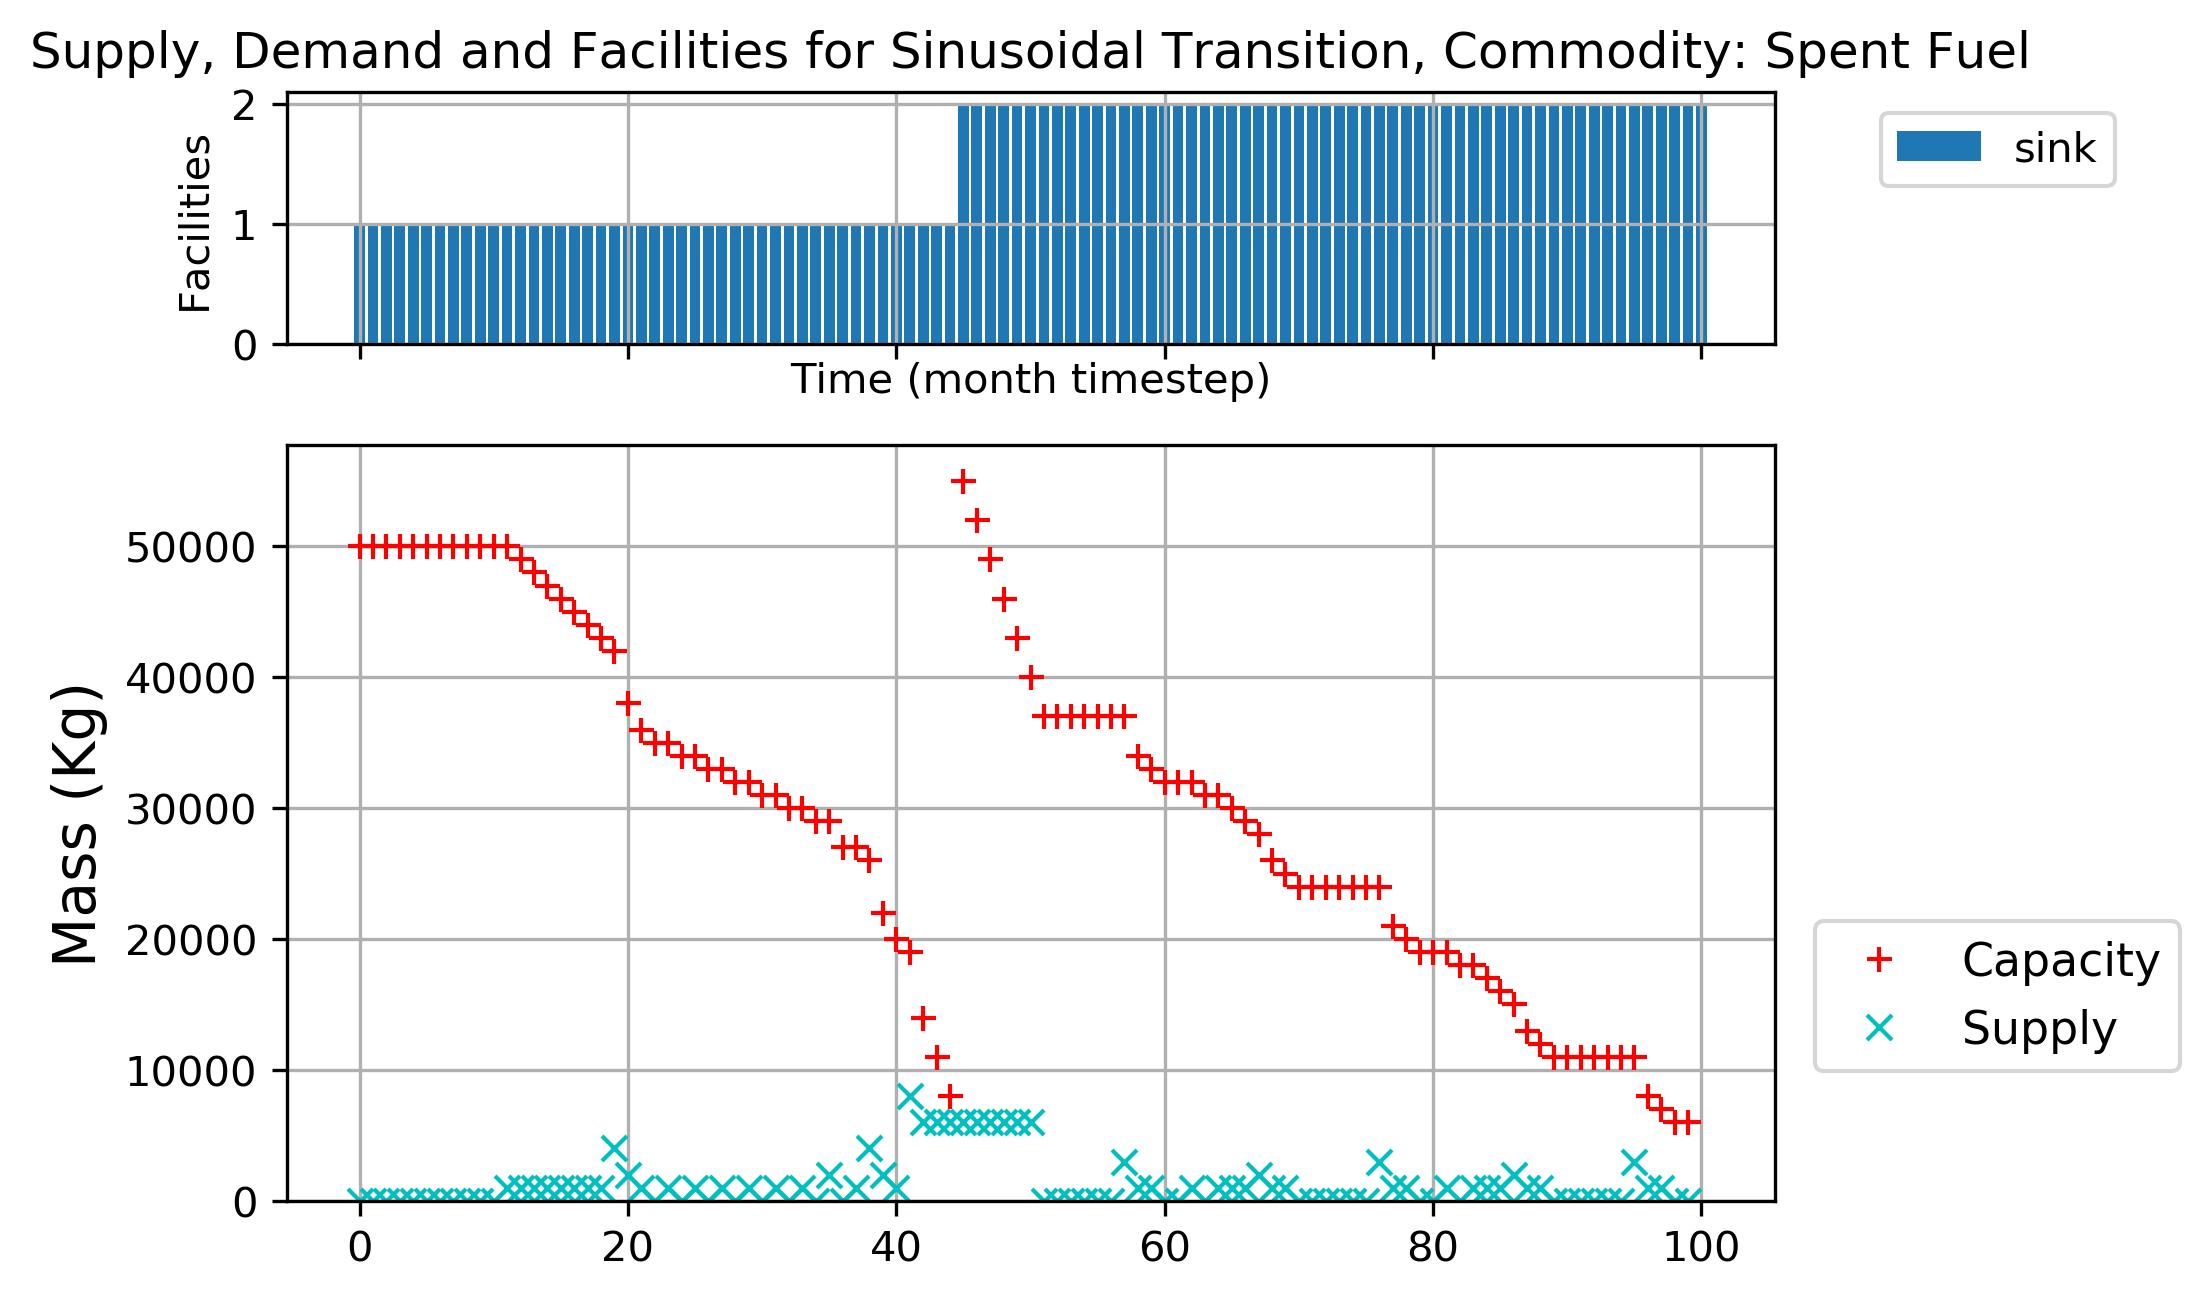
\includegraphics[width=0.9\linewidth]{figures/sinetransition-spentfuel.png} 
            \caption{Spent fuel demand and supply, and sink facility deployment plot.
                Spent fuel is supplied by reactors and the capacity to store them 
                is provided by sink facilities.
            There are no time steps with under-capacity of sink space \cite{chee_arfc/transition-scenarios_2018}.}
            \label{fig:sinetransition-spentfuel}
        \end{subfigure}
        \caption{Simple sinusoidal power demand transition scenario with 
        three facility types: \texttt{source}, \texttt{reactor}, and \texttt{sink}.}
    \end{figure}

    \begin{table}[]
        \centering
        \doublespacing
        \caption {The total number of time steps with commodity undersupply 
        for each simple transition scenario. }
        \label{tab:transition-scenario-results}
            \small
            \begin{tabular}{l|rr}	
                \hline
                \textbf{Simple Transition Scenario}    & \textbf{Commodity}    & \textbf{Undersupplied} \\ 
                && \textbf{time steps [\#] } \\ \hline
                \multirow{3}{*}{\textbf{Constant Power}} & Fuel & 1 \\ 
                                                         & Power & 0 \\ 
                                                         & Spent Fuel & 0 \\ \hline
                \multirow{3}{*}{\textbf{Linearly Increasing Power}} & Fuel & 1 \\ 
                                                         & Power & 0 \\ 
                                                         & Spent Fuel & 0 \\ \hline
                \multirow{3}{*}{\textbf{Sinusoidal Power}} & Fuel & 1 \\ 
                                                         & Power & 1 \\ 
                                                         & Spent Fuel & 0 \\ \hline
                \end{tabular}
    \end{table}

\section{\deploy Demonstration of EG01-30 Transition Scenario} 
\label{sec:eg01-30}
In this section, we use \deploy to set up the transition scenario from 
the current once through LWR fuel cycle (EG01) to a closed fuel cycle 
with continuous recycling of U/TRU in fast and thermal spectrum 
reactors (EG30). 
EG30 is one of the promising nuclear fuel cycles identified by DOE's 
evaluation and screening study (described in Section \ref{sec:egs}).

Figure \ref{fig:30flow} shows the setup of facilities and mass flows 
for EG01-30 in \Cyclus. 
In the EG01-30 transition scenario, the initial LWR fleet 
progressively decommissions at the 80-year mark,
after which \deploy deploys \glspl{SFR} and \gls{MOX} \glspl{LWR} to 
meet a linearly increasing power demand. 
Transuranic elements from the spent fuel are recycled to 
produce \gls{MOX} \gls{LWR} and \gls{SFR} fuel. 
The power demand equation: 
\begin{align}
    P(t) &= 60000 + \frac{250t}{12} \\ 
    \intertext{where:}
    t &= \mbox{time step [month]} \nonumber \\
    P(t) &= \mbox{time-dependent power [MW]} \nonumber
\end{align}

\begin{figure}[]
	\centering
    \begin{tikzpicture}[node distance=2.5cm]
    \tikzstyle{every node}=[font=\normalsize]
    \node (source)[ollblock]{\texttt{Source}};
    \node (enrich)[ollblock, below of=source]{\texttt{Enrichment}};
    \node (lwr)[ollblock, below of=enrich]{\texttt{LWR}};
    \node (lwrsto)[ollblock, below of=lwr]{\texttt{LWR Cooling Pool}};
    \node (lwrrep)[ollblock, below of=lwrsto]{\texttt{LWR Reprocessing}};
    \node (lwrrepo)[ollblock, below of=lwrrep]{\texttt{LWR Waste Repository}};
    \node (frmix)[ollblock, right of=enrich, xshift=3cm]{\texttt{FR Mixer}};
    \node (fr)[ollblock, right of=lwr, xshift=3cm]{\texttt{FR}};
    \node (frsto)[ollblock, right of=lwrsto, xshift=3cm]{\texttt{FR Cooling Pool}};
    \node (frrep)[ollblock, right of=lwrrep, xshift=3cm]{\texttt{FR Reprocessing}};
    \node (frrepo)[ollblock, right of=lwrrepo, xshift=3cm]{\texttt{FR Waste Repository}};
    \node (moxmix)[ollblock, right of=frmix, xshift=3cm]{\texttt{MOX Mixer}};
    \node (mox)[ollblock, right of=fr, xshift=3cm]{\texttt{MOX LWR}};
    \node (moxsto)[ollblock, right of=frsto, xshift=3cm]{\texttt{MOX Cooling Pool}};
    \node (moxrep)[ollblock, right of=frrep, xshift=3cm]{\texttt{MOX Reprocessing}};
    \node (moxrepo)[ollblock, right of=frrepo, xshift=3cm]{\texttt{MOX Waste Repository}};
    \path[->] (source) edge[line width=0.5mm] node[ fill=white, anchor=center, pos=0.5] {natl-U} (enrich);
    \path[->] (enrich) edge[line width=0.5mm] node[ fill=white, anchor=center, pos=0.5] {LWR fuel} (lwr);
    \path[->] (lwr) edge[line width=0.5mm] node[ fill=white, anchor=center, pos=0.5] {LWR used fuel} (lwrsto);
    \path[->] (lwrsto) edge[line width=0.5mm] node[ fill=white, anchor=center, pos=0.5] {\shortstack{cooled used \\ LWR fuel}} (lwrrep);
    \path[->] (lwrrep) edge[line width=0.5mm] node[ fill=white, anchor=center, pos=0.5] {\shortstack{LWR reprocessing \\ waste}} (lwrrepo);
    \path[->] (frmix) edge[line width=0.5mm] node[ fill=white, anchor=center, pos=0.5] {FR fuel} (fr);
    \path[->] (fr) edge[line width=0.5mm] node[ fill=white, anchor=center, pos=0.5] {FR used fuel} (frsto);
    \path[->] (frsto) edge[line width=0.5mm] node[ fill=white, anchor=center, pos=0.5] {\shortstack{cooled used \\ FR fuel}} (frrep);
    \path[->] (frrep) edge[line width=0.5mm] node[ fill=white, anchor=center, pos=0.5] {\shortstack{FR reprocessing \\ waste}} (frrepo);
    \path[->] (moxmix) edge[line width=0.5mm] node[ fill=white, anchor=center, pos=0.5] {MOX fuel} (mox);
    \path[->] (mox) edge[line width=0.5mm] node[ fill=white, anchor=center, pos=0.5] {MOX used fuel} (moxsto);
    \path[->] (moxsto) edge[line width=0.5mm] node[ fill=white, anchor=center, pos=0.5] {\shortstack{cooled used \\ MOX fuel}} (moxrep);
    \path[->] (moxrep) edge[line width=0.5mm] node[ fill=white, anchor=center, pos=0.5] {\shortstack{MOX reprocessing \\ waste}} (moxrepo);
    \draw [arrow] (lwrrep) -- ([shift={(0.7cm,0cm)}]lwrrep.east)-- node[ fill=white, anchor=center, pos=0.5] {U/TRU} ([shift={(-0.7cm,0cm)}]frmix.west)--(frmix);
    \draw [arrow] (frmix) -- ([shift={(-0.7cm,0cm)}]frmix.west) |- ([shift={(0cm,0.9cm)}]moxmix.north)--(moxmix);
    \draw [arrow] (frrep) -- ([shift={(0.7cm,0cm)}]frrep.east)-- node[ fill=white, anchor=center, pos=0.5] {U/TRU} ([shift={(0.7cm,0cm)}]frmix.east)--(frmix);
    \draw [arrow] (frmix) -- ([shift={(0.7cm,0cm)}]frmix.east) |- ([shift={(-0.7cm,0cm)}]moxmix.west)--(moxmix);
    \draw [-,thick] (moxrep) -- ([shift={(-0.7cm,0cm)}]moxrep.west)-- ([shift={(0.7cm,0cm)}]frrep.east)--(frrep);
\end{tikzpicture}
	
    \caption{Facility and mass flow for the EG01-EG30 transition scenario.
    EG01 is the current once through LWR fuel cycle.
    EG30 is a closed fuel cycle 
    with continuous recycling of U/TRU in fast and thermal reactors.}
    \label{fig:30flow}
\end{figure}

We compared different prediction 
methods and power supply buffer sizes to determine the 
optimal \deploy parameters for minimizing
power undersupply in the EG01-30 \Cyclus 
transition scenario. 
The subsequent sections discuss the results from the comparison 
study. 

\subsection{Comparison of Prediction Methods}
We ran EG01-30 transition scenarios with different prediction 
methods to determine the prediction method that best minimizes 
power undersupply. 
In Figure \ref{fig:eg30under}, each histogram represents 
the number of time steps with undersupply or 
under capacity for all commodities for each prediction method.  
Table \ref{tab:all-power} shows the number of time steps with power 
undersupply for the linearly increasing power EG01-30 transition scenario. 
Figure \ref{fig:eg30under} and Table \ref{tab:all-power}
demonstrate that the \texttt{FFT} and \texttt{POLY} methods 
perform the best for the EG01-30 transition scenario, 
with the fewest time steps with power undersupply.

\begin{figure}[]
	\centering
	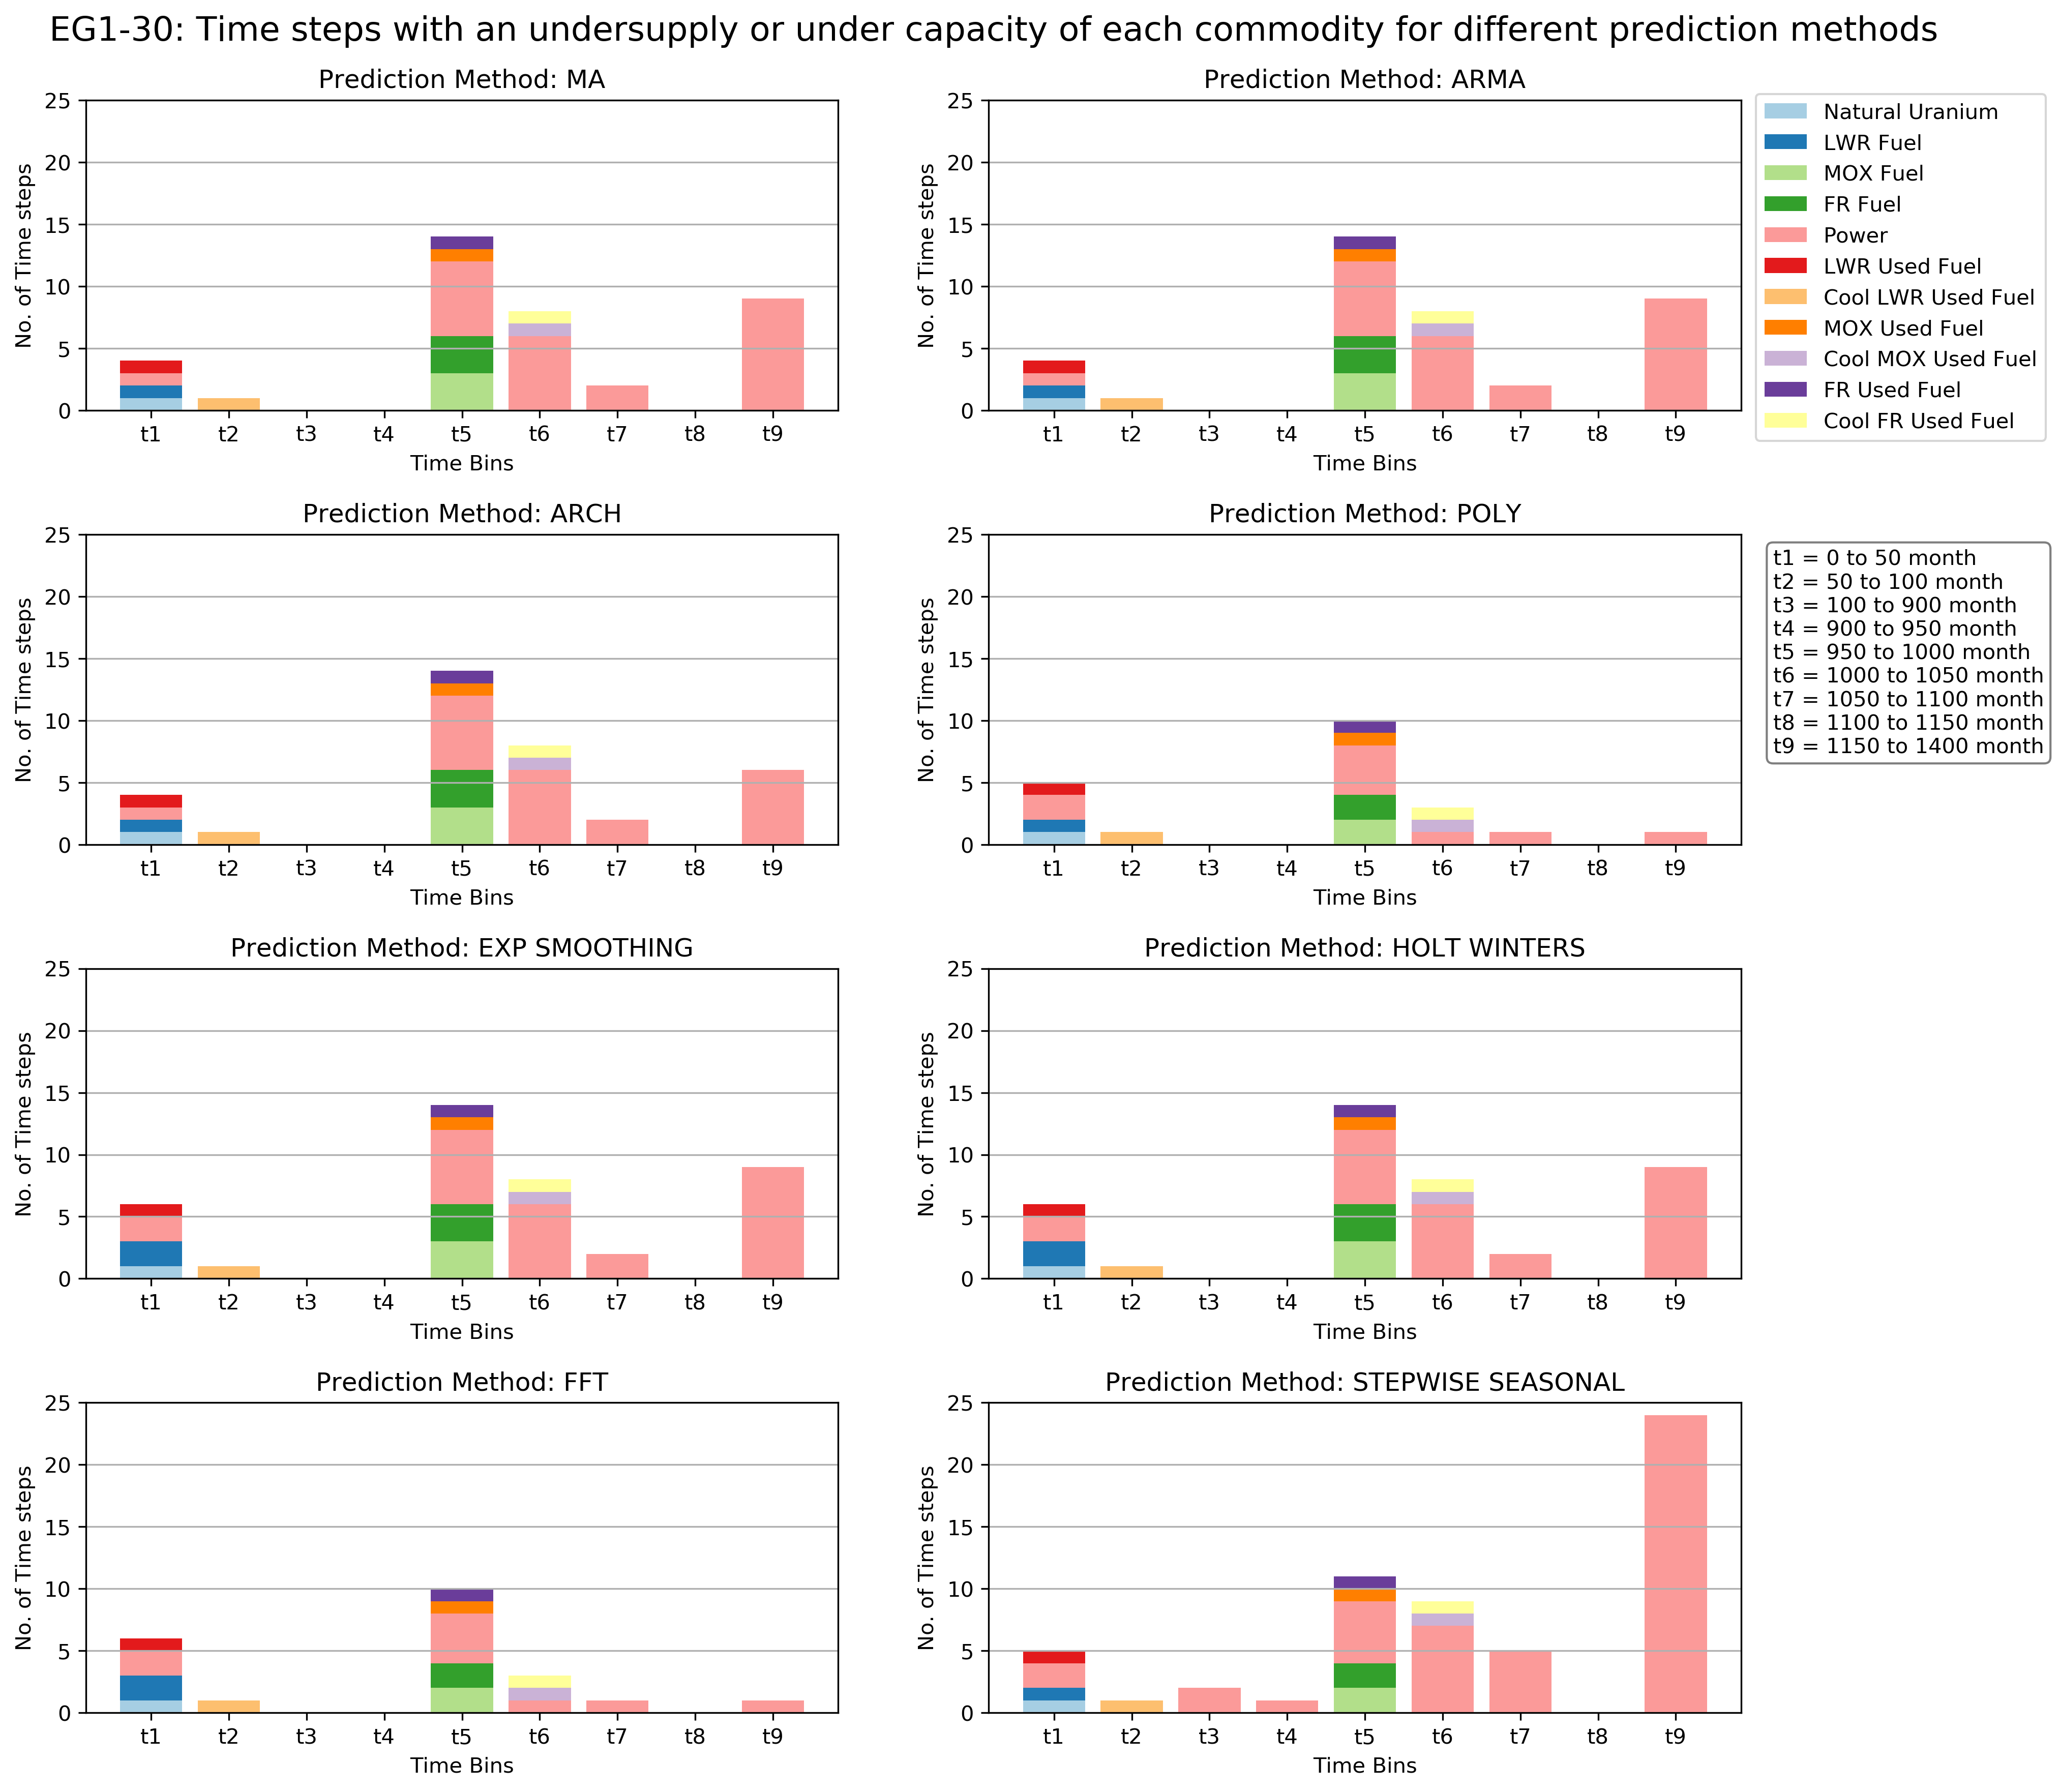
\includegraphics[width=0.88\linewidth]{eg01-30-histogram.png} 
	\caption{
	EG01-30 transition scenario with linearly increasing power demand. 
	Each subplot shows the total number of time steps in which there exists 
	undersupply and under capacity of commodities for each prediction method. 
	The different colors represent different commodities, and each vertical bar
	refers to 50 time steps in the simulation.
    The \texttt{FFT} and \texttt{POLY} prediction methods perform the best, 
    with the fewest
	time steps with undersupply and undercapacity \cite{chee_arfc/transition-scenarios_2018}.}
	\label{fig:eg30under}
\end{figure}

\begin{table}[]
    \doublespacing
	\centering
        \caption{Total number of time steps with power undersupply for the 
        EG01-30 transition scenario for different prediction methods.}
		\label{tab:all-power}
		\small
        \begin{tabular}{lr}
		\hline
        \textbf{Algorithm} & \textbf{EG01-30: No. of Time Steps} \\ 
        & \textbf{with Power Undersupply} \\ \hline
		\texttt{MA}     		& 24 \\ 
		\texttt{ARMA}     	    & 24\\ 
		\texttt{ARCH}     	    & 21\\ 
		\texttt{POLY}      		&  9\\ 
		\texttt{EXP-SMOOTHING} 	& 25\\ 
		\texttt{HOLT-WINTERS}  	& 25\\ 
		\texttt{FFT}       		& 9\\ 
		\texttt{SW-SEASONAL}    & 51\\ \hline
	\end{tabular}
\end{table}


\subsection{Comparison of Power Buffer Sizes}
For the EG01-30 linearly increasing power demand 
transition scenario, the power buffer size is varied
for both \texttt{FFT} and \texttt{POLY} methods. 
Varying the power buffer size does not impact the number of 
undersupplied time steps for the transition scenario 
with the \texttt{POLY} prediction method.
For the transition scenario with \texttt{FFT} prediction method, 
Figure \ref{fig:eg30-bufplot} and Table \ref{tab:buff_size} 
show that with increased buffer size, the number of 
power undersupply time steps decreases. 
The cumulative undersupply is minimized with an 8000MW 
buffer.
However, this means 8 extra reactors are required, which 
is unrealistic.
In Figure \ref{fig:eg30-bufplot}, a 2000MW buffer size has 
6 time steps with undersupply, while a 8000MW buffer size has 
5 time steps with undersupply. 
The extra commissioning of 6 reactors does not justify the 1 time 
step. 
For a 2000MW buffer size simulation, undersupply time 
steps occur at the beginning of the simulation and for two 
time steps when the transition begins. 
This is expected since without time series data 
at the beginning of the simulation, \deploy takes a few 
time steps to collect time series data about power demand 
to predict and start deploying reactor and supporting 
fuel cycle facilities. 
In reality, the power undersupply during the transition 
can be filled by coordinating refueling or short-term use of 
alternative energy sources.  
Therefore, a buffer of 2000MW minimizes 
the power undersupply for the EG01-EG30 transition scenario
with the \texttt{FFT} prediction method.

\begin{figure}[]
		\centering
		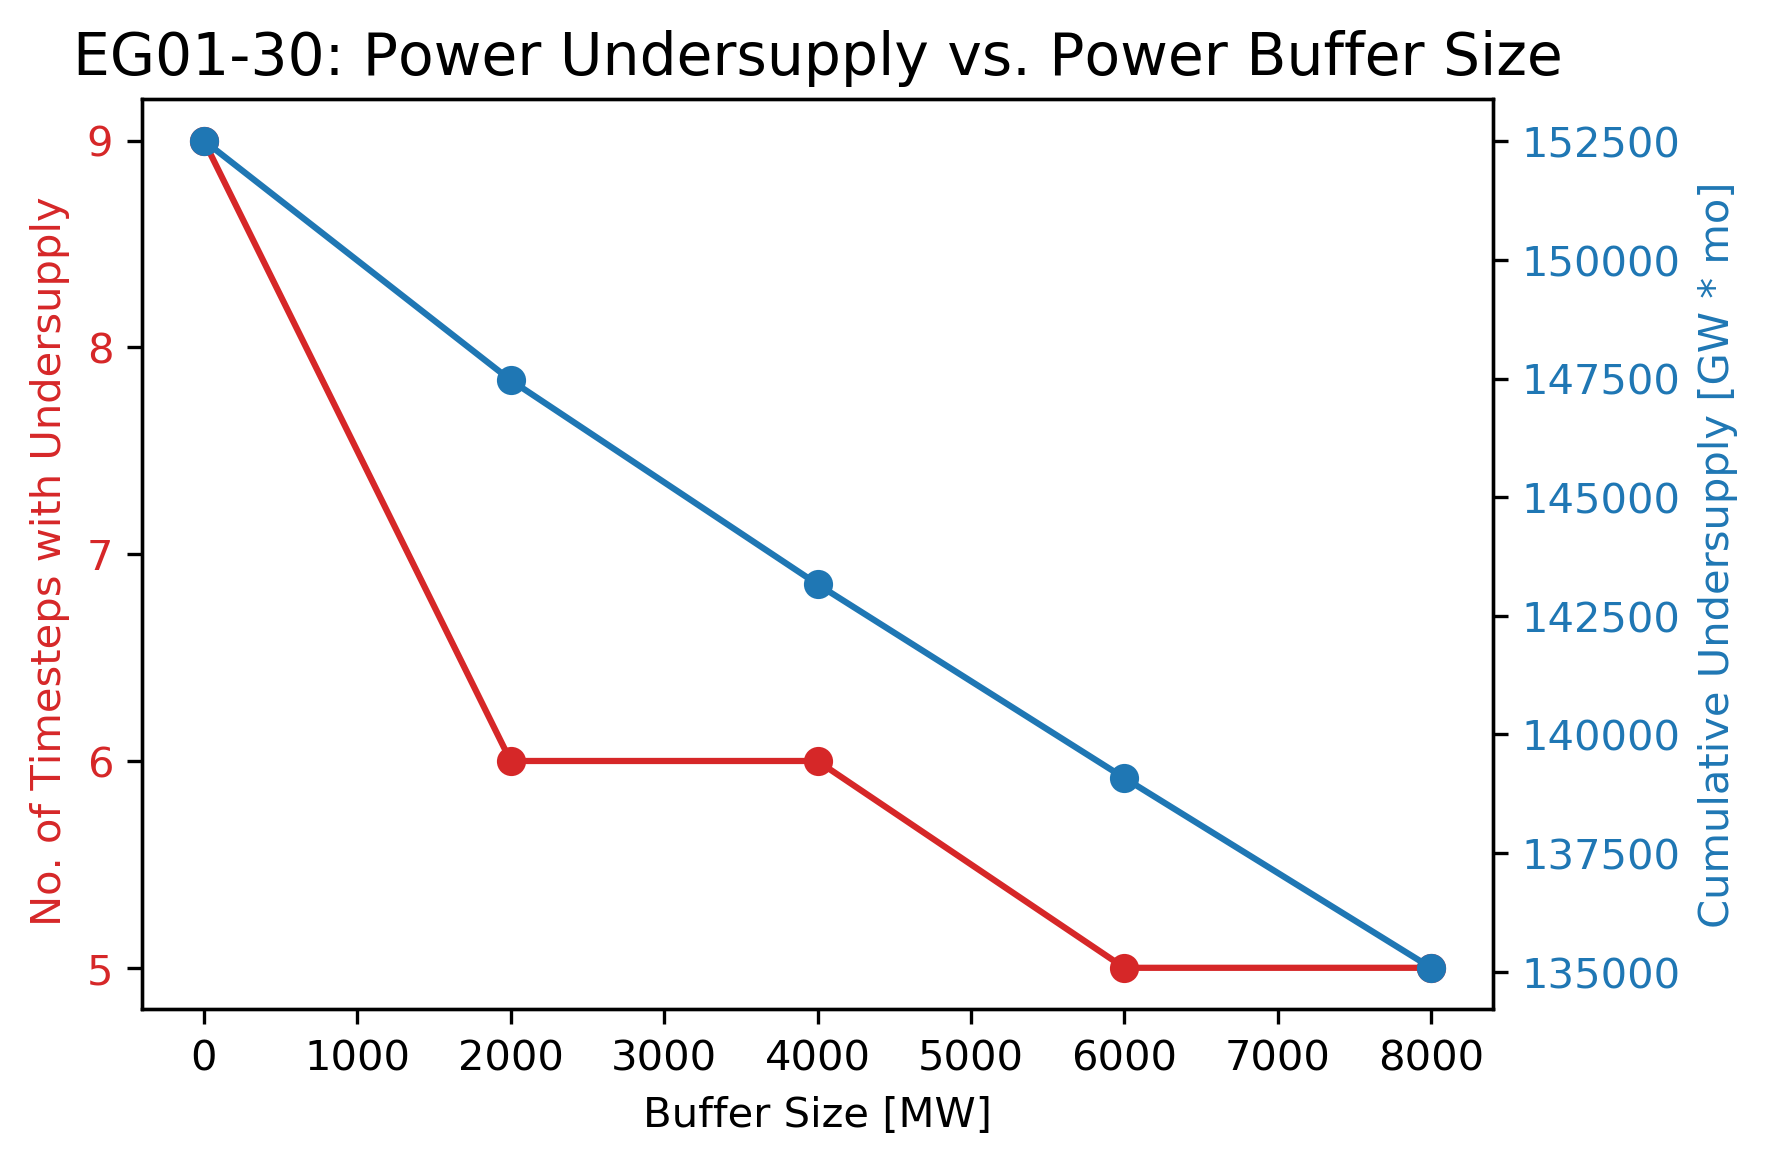
\includegraphics[width=\linewidth]{30-sens-buffer.png} 
    \caption{The effect of power buffer size on 
    power undersupply for the EG01-30 transition scenario with linearly 
    increasing power demand using the \texttt{FFT} method.}
    \label{fig:eg30-bufplot}
\end{figure}

\begin{table}[h]
    \centering
    \doublespacing
	\caption{Dependency of the power undersupply on the buffer size 
	for EG01-EG30 transition scenarios with linearly 
    increasing power demand using the \texttt{FFT} prediction method.
    There is less power undersupply for a larger power buffer size.}
	\label{tab:buff_size}
	\small
	\begin{tabular}{rrr}
                \hline
                \textbf{Buffer [MW]}     & \textbf{Undersupply}               & \textbf{EG01-30} \\
		\hline
		\textbf{0}             & Time steps $[\#]$  & 9\\  
                      & Cumulative $[GW\cdot mo]$    & 152517 \\ \hline
        \textbf{2000}          & Undersupplied $[\#]$ & 6 \\  
        	      & Cumulative $[GW\cdot mo]$   & 147166 \\ \hline
        \textbf{4000}         & Time steps $[\#]$ & 6 \\  
				  & Cumulative $[GW\cdot mo]$     & 143166 \\ \hline
        \textbf{6000}          & Time steps $[\#]$  & 5 \\  
		& Cumulative $[GW\cdot mo]$     & 139083 \\ \hline
        \textbf{8000}          & Time steps $[\#]$  & 5  \\  
	              & Cumulative $[GW\cdot mo]$  & 135083 \\ \hline
	\end{tabular}
\end{table}

\subsection{Demonstration of Best Performance Model}
Table \ref{tab:bestinputs} 
shows \deploy input parameters for the 
EG01-EG30 transition scenario
that minimize undersupply of power and minimize 
the undersupply and under capacity of the other commodities
in the simulation. 
The need for commodity buffers reflects reality
in that a supply buffer is usually maintained to ensure 
continuity in the event of an unexpected failure in the supply chain.

Figure \ref{fig:30stack} shows the
time-dependent deployment of reactors and supporting facilities 
for the EG01-30 linearly increasing power demand 
transition scenario in which \glspl{LWR} transition to 
\gls{MOX} \glspl{LWR} and \glspl{SFR}.

\begin{table}[]
    \centering
    \doublespacing
    \caption{\deploy's input parameters for the
	EG01-EG30 transition scenario
	which minimize undersupply for power and minimizes 
	the undersupply and under capacity for other facilities. }
	\label{tab:bestinputs}
    \small
    \begin{tabular}{llr}
    \hline
                              & \textbf{\deploy Input Parameter}            & \textbf{EG01-30}            \\ \hline
    \multirow{4}{*}{\textbf{Required}} & Demand driving commodity   & Power              \\
                              & Demand equation {[}MW{]}   & 60000+250t/12        \\
                              & Prediction method          & \texttt{FFT}                \\
                              & Deployment driving method  & Installed Capacity \\ \cline{1-3}
    \multirow{2}{*}{\textbf{Optional}} & Buffer type                & Absolute           \\
                              & Power buffer size {[}MW{]} & 2000               \\ 
                              & Transition start date [Month] & 960 (Year 80)\\ 
                              & Fleet share percentage [\%] & MOX LWR: 15\%, \gls{SFR}: 85\%\\ \hline
    \end{tabular}%
    \end{table}

    \begin{figure}[]
        \centering
        \begin{subfigure}[t]{\textwidth}
            \centering
            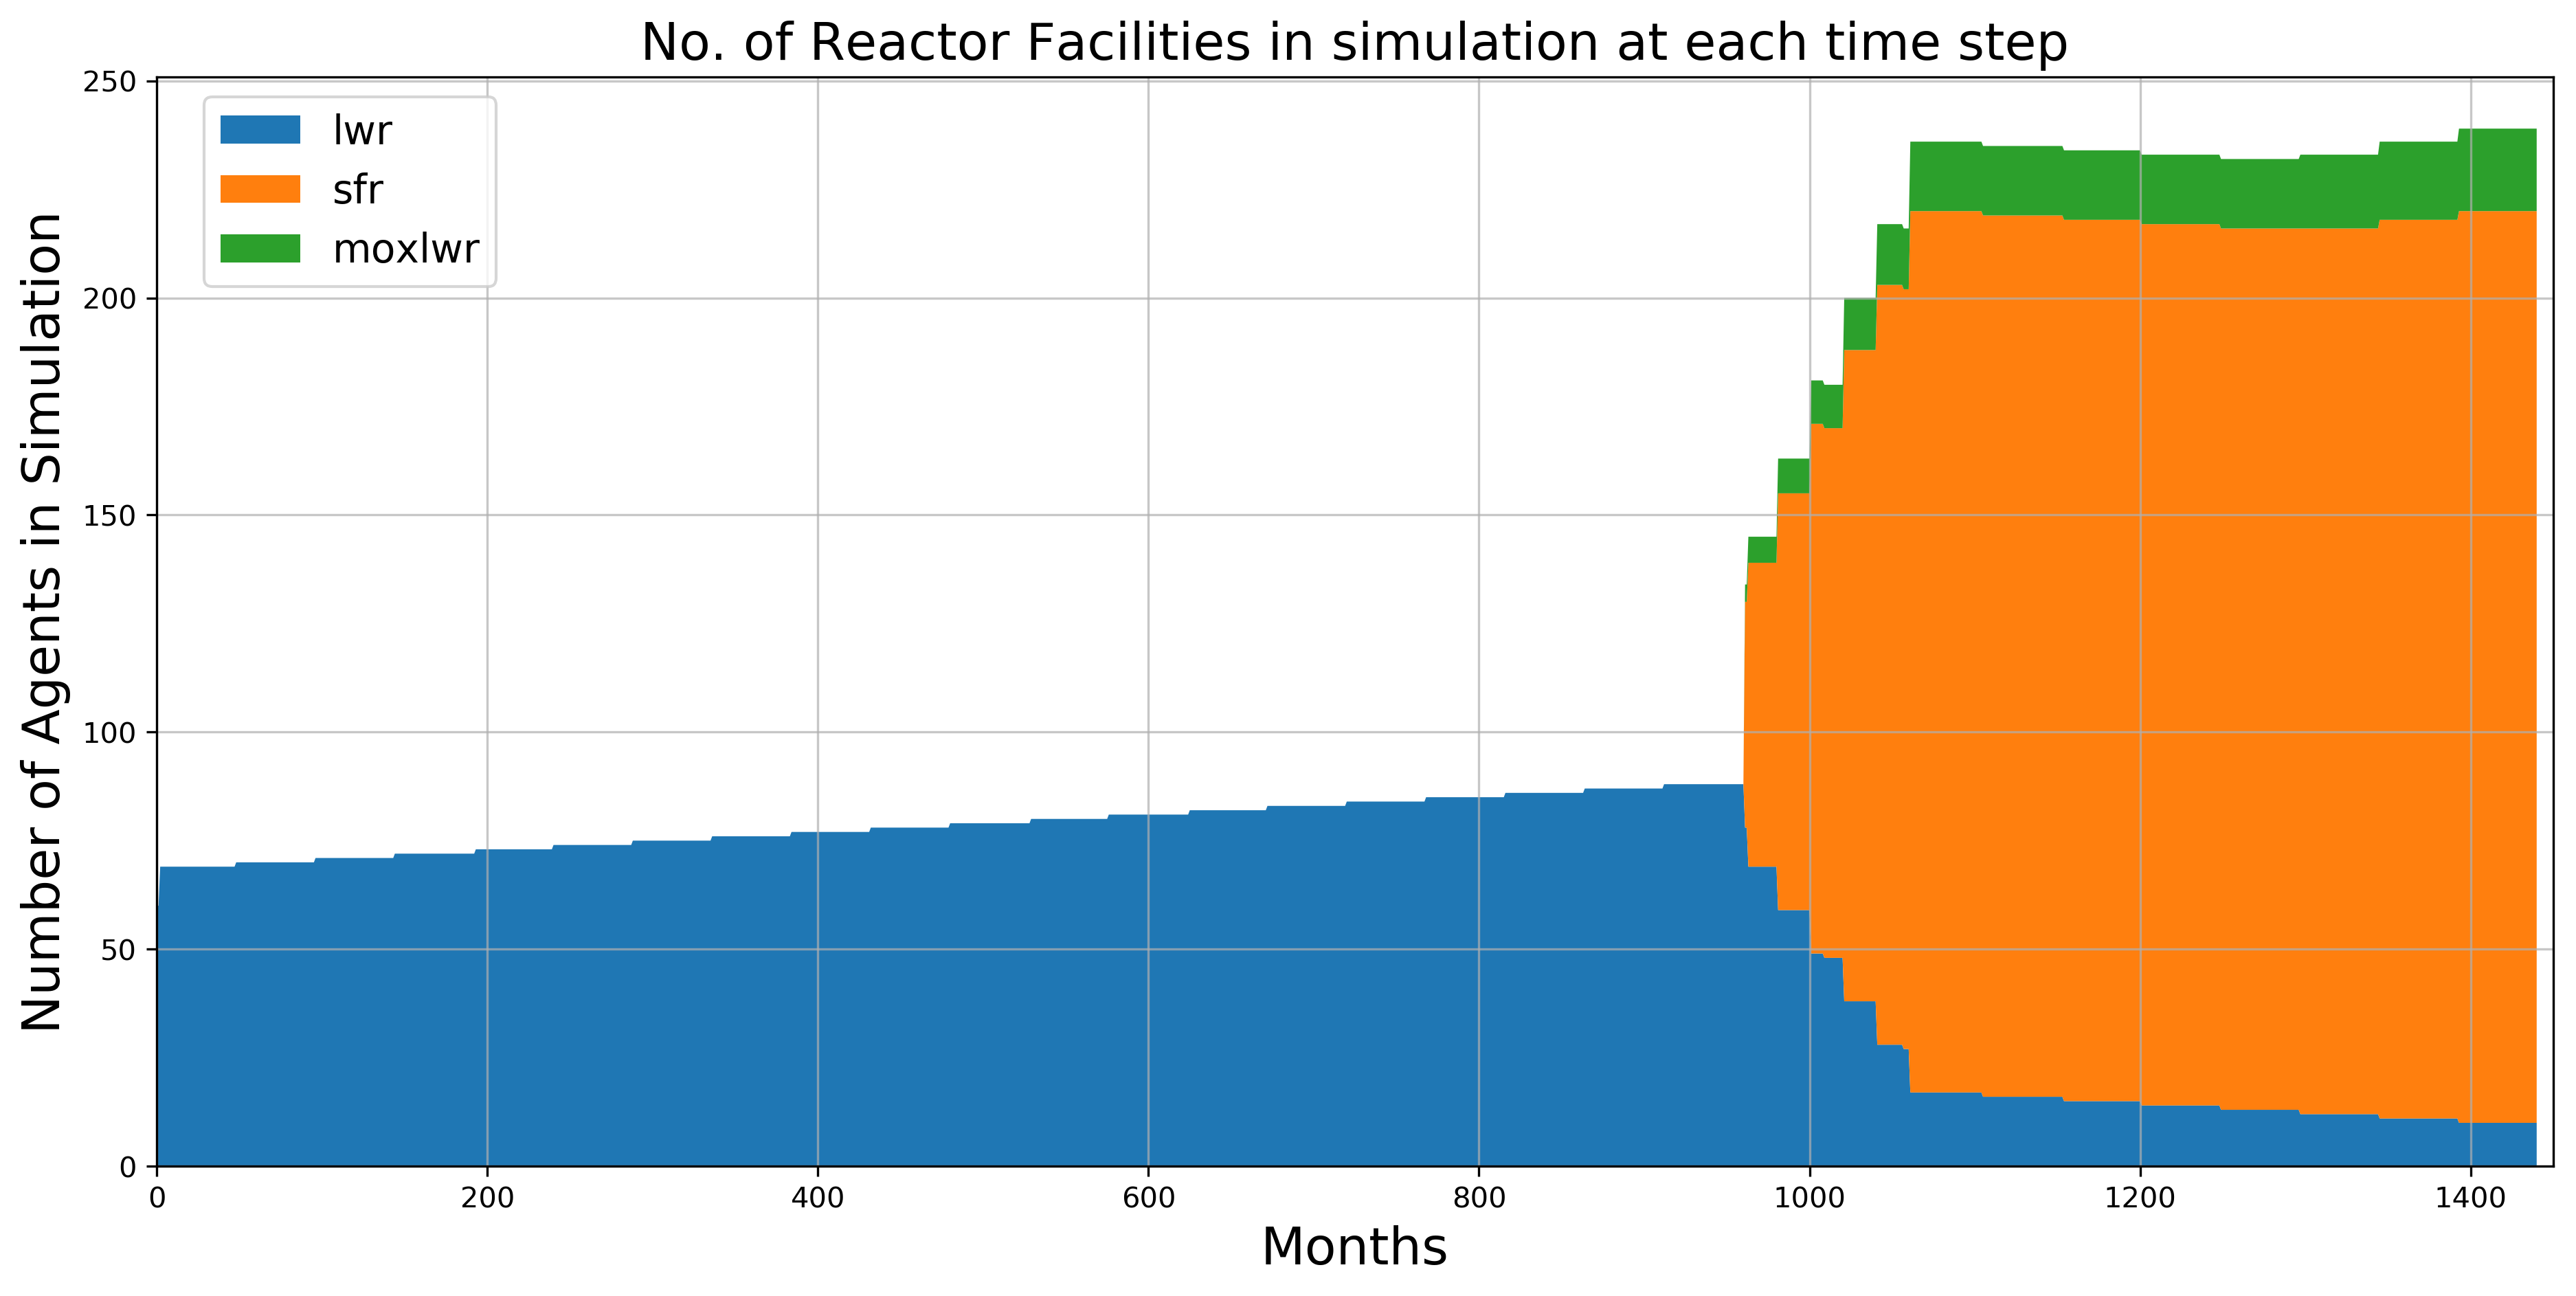
\includegraphics[width=\linewidth]{eg30-stack_reactor.png} 
            \caption{EG01-30: Reactor Deployment}
            \label{fig:30reactor}
        \end{subfigure}
        \vspace{1cm}
        \begin{subfigure}[t]{\textwidth}
            \centering
            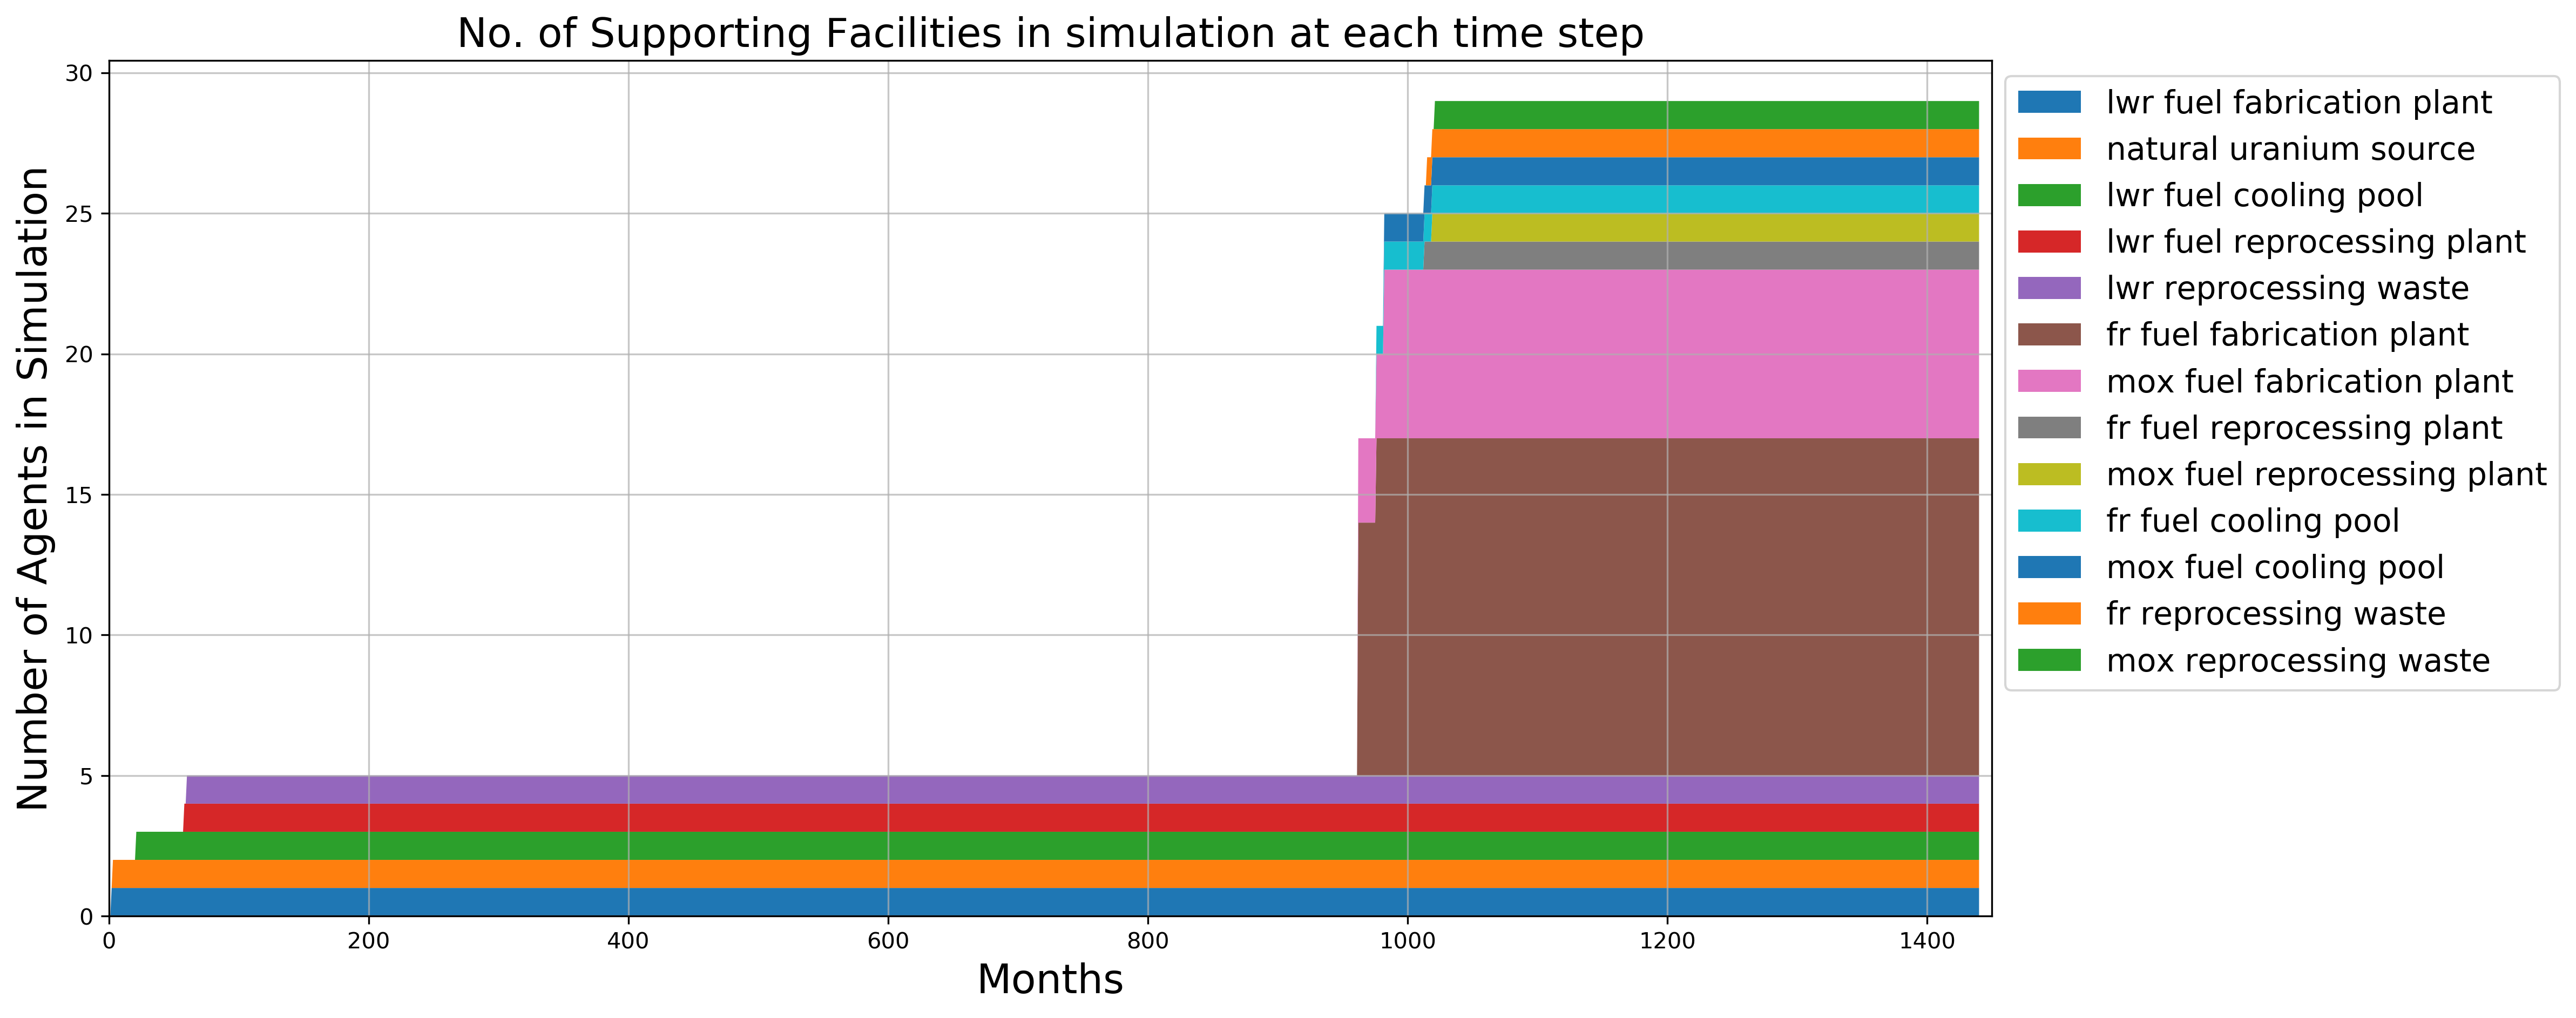
\includegraphics[width=\linewidth]{eg30-stack_support.png} 
            \caption{EG01-30: Supporting Facility Deployment}
            \label{fig:30support}
        \end{subfigure}
        \hfill
        \caption{Time dependent deployment of reactor and supporting facilities in 
        the EG01-30 linearly increasing power demand transition scenario. 
        \deploy automatically deploys reactor and supporting facilities 
        to setup a supply chain to meet linearly increasing power demand of $60000 + 250t/12$ MW
        during a transition from \glspl{LWR} to MOX LWRs and \glspl{SFR} \cite{chee_arfc/transition-scenarios_2018}. }
        \label{fig:30stack}
    \end{figure}

\section{Chapter Summary}
In this chapter, we demonstrate \deploy's automatic deployment of 
fuel cycle facilities to meet constant, linearly increasing, 
and sinusoidal power demand in simple three-facility transition 
scenarios. 
Knowing that \deploy works for simple transition scenarios, 
we use \deploy to set up a complex transition from the current once through 
LWR fuel cycle (EG01) to a closed fuel cycle 
with continuous recycling of U/TRU in fast and thermal spectrum 
reactors (EG30).
We demonstrate that \deploy can automatically deploy fuel cycle facilities to 
meet a linearly increasing power demand in the EG01-EG30 
transition scenario. 
In the next chapter, \deploy ensures automatic transition set up for 
sensitivity analysis studies of this EG01-30 transition scenario. 

